\chapter{Estudi d'Experiència d'Usuari (UX)}

\section{Anàlisi}
L'objectiu d'aquest apartat és definir com seran els usuaris potencials de l'aplicació. Per a fer-ho s'analitzarà com interaccionen amb les aplicacions de gestió de despeses per extreure les necessitats i els requeriments del producte.

\subsection{Investigació contextual}
En aquesta secció s'ha estudiat com els usuaris gestionen les despeses. Per a fer-ho, s'han entrevistat 9 usuaris sobre com gestionen actualment les seves despeses, demanant que mostressin com ho feien. A més a més, a 4 d'aquests 9 usuaris se'ls ha demanat que utilitzessin varies aplicacions ja existents al mercat (\gls{Google_play}). Un cop les feien servir en directe se'ls preguntava quines coses els havien agradat i quines no. 
%TODO link apps

La totalitat de l'entrevista ha estat transcrita al moment i conduïda per la plantilla de la figura \ref{fig:plantilla_analisi}. És important remarcar que tot i ser una entrevista es buscava, sempre que era possible, que els usuaris mostressin com treballen, enlloc de que expliquessin amb paraules com ho fan. També, quan els usuaris utilitzaven les aplicacions s'ha gravat un vídeo amb el què veien a la pantalla mentre feien servir les aplicacions així com el que poguessin estar dient en aquell moment. L'objectiu de fer aquestes gravacions és facilitar, si s'escau, el posterior anàlisi per aclarir parts de l'enquesta que no fossin prou clars. Al comptar amb so, també ha servit per localitzar i identificar les funcions o apartats que frustraven o motivaven als usuaris. Per últim, quan ha estat possible s'han recol·lectat imatges o documents que ensenyessin com els usuaris gestionen les seves despeses i/o ingressos. 

\begin{figure}[htp]
\centering
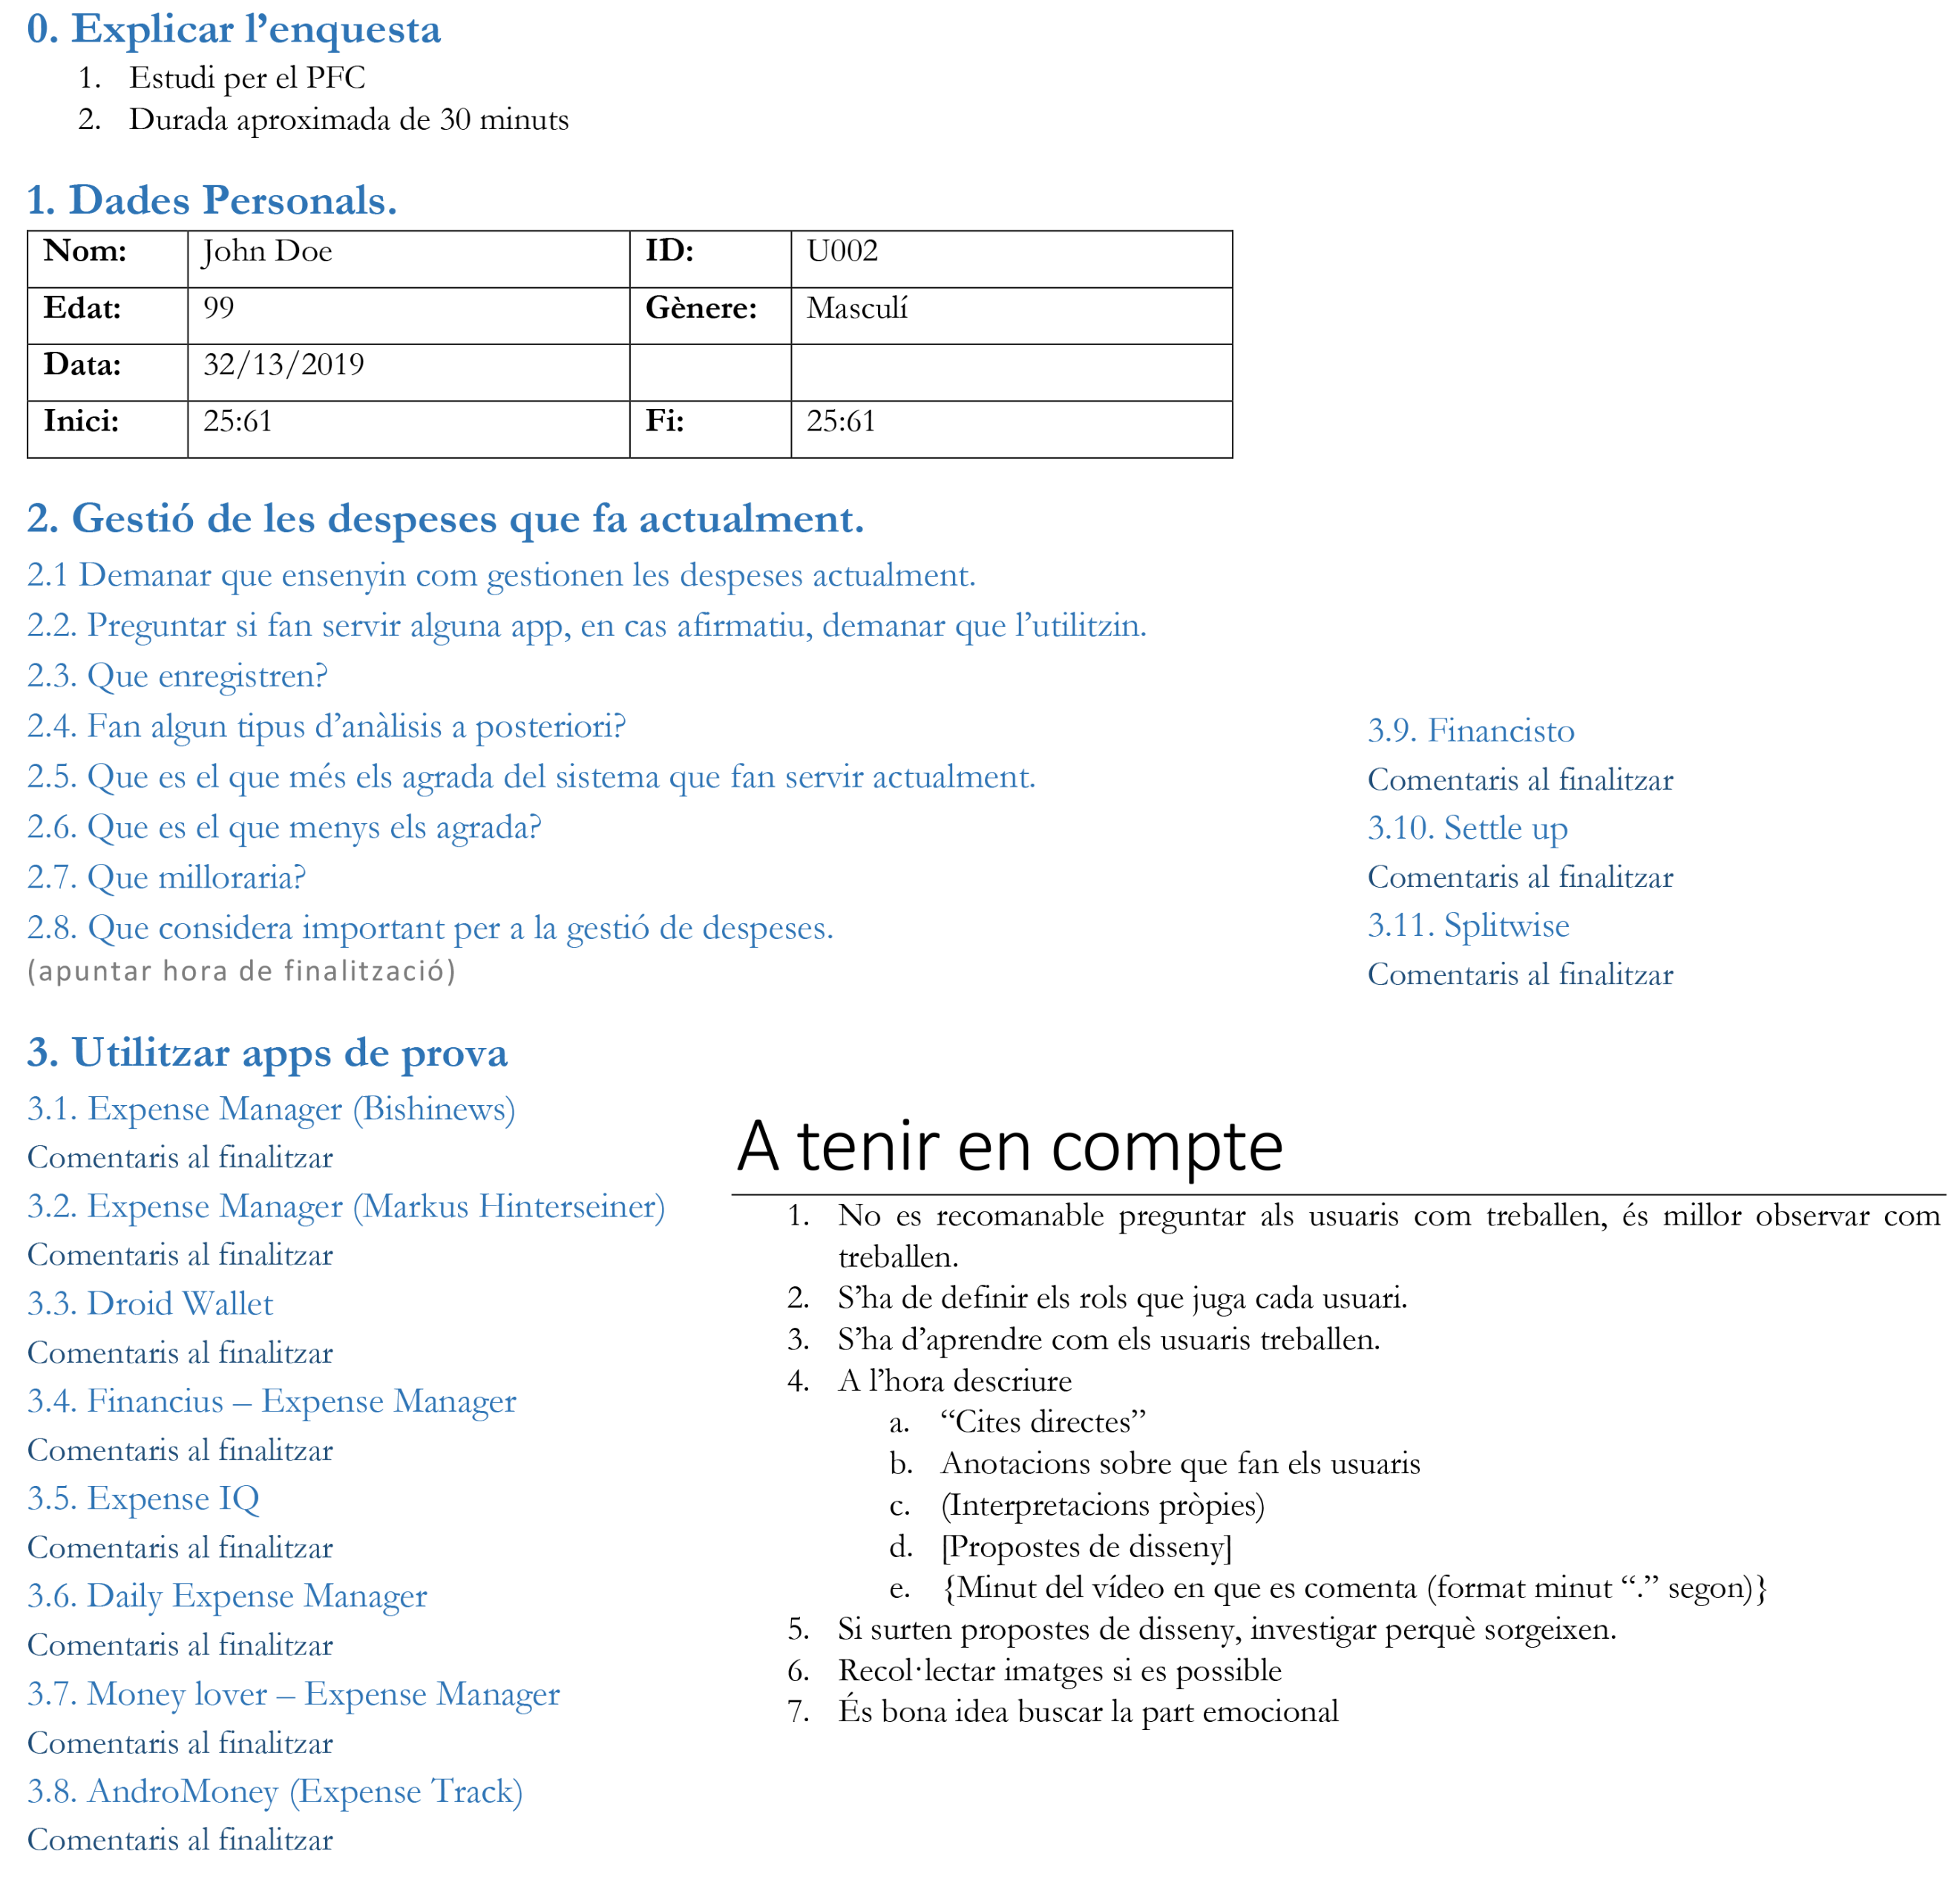
\includegraphics[scale=0.65]{plantilla_analisi.png}
\caption{Plantilla emprada a la investigació contextual}\label{fig:plantilla_analisi}
\end{figure}

\subsection{Anàlisi contextual}
En aquesta secció s'ha creat el model de flux (figura \ref{fig:flow_model}). També s'ha sintetitzat la informació extreta a la investigació contextual en \glspl{workActivityNotes}. Després amb les \glspl{workActivityNotes} s'ha creat el \ac{WAAD}, de manera que aquest mostra de manera clara i concisa la informació que s'ha extret dels usuaris. Cada \gls{workActivityNotes} dins del \ac{WAAD} està etiquetada amb el numero de nota i un identificador (format per lletres i números) que la posiciona dins el \ac{WAAD}.

%TODO link del WAAD

\begin{figure}[htp]
\centering
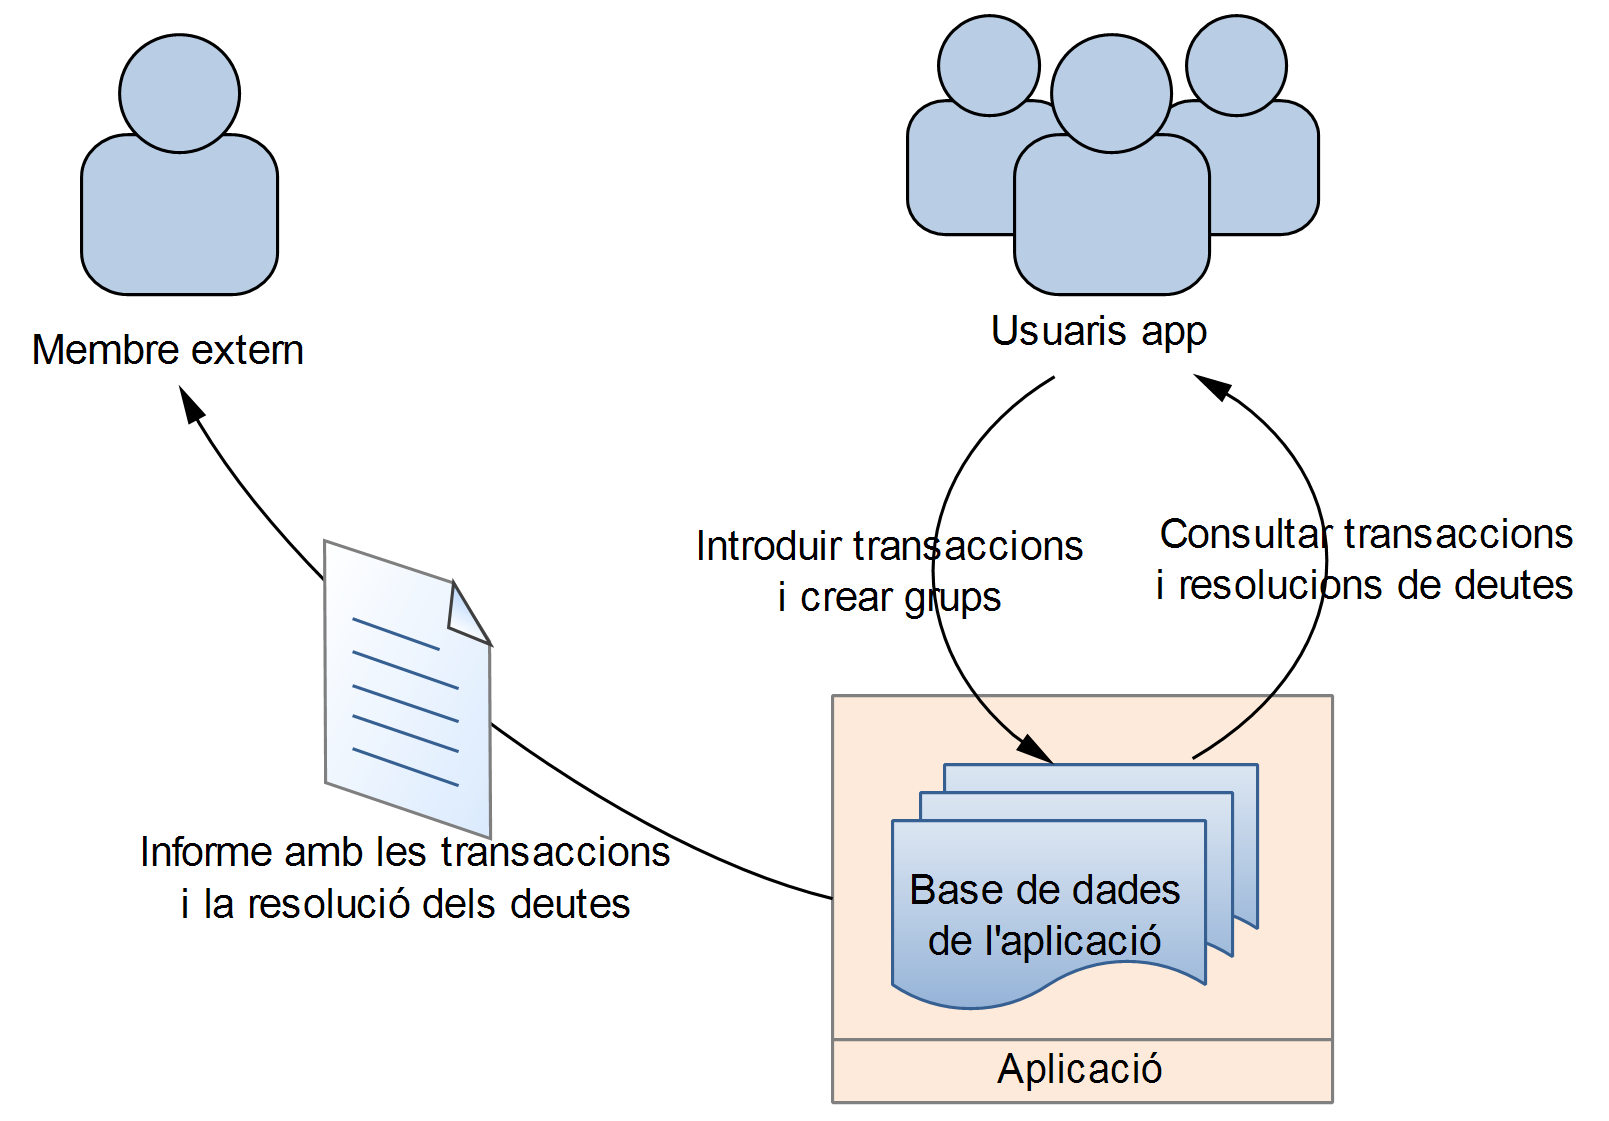
\includegraphics[scale=0.5]{flow_model.png}
\caption{Model de flux}\label{fig:flow_model}
\end{figure}

\subsection{Extracció dels requeriments d'interacció}
Aquí s'han extret els requeriments d'interacció a partir del \ac{WAAD}. A més a més, tal com recomana Rex Hartson (2012, p.168) \cite{UX_Book} també s'han inclòs de color verd els requeriments del sistema. S'han marcat amb un triangle (\blacktriangle) els requeriments més importants per tal de ressaltar-ne la seva importància. També, com que sovint l'usuari no menciona les coses que considera obvies, s'han extrapolat aquells requeriments que no estaven mencionats directament però que els usuaris esperen. 
Per últim, per a poder localitzar la font de cada requeriment, s'ha etiquetat entre claudàtors l'identificador del \ac{WAAD} de la \gls{workActivityNotes} de la qual prové.

\subsection{Construcció de models informatius per al disseny}
En aquesta secció s'han creat els diversos models descrits a l'apartat \ref{subsubsec:Construccio_models}.
Tot i això, com que el producte que s'està dissenyant és una aplicació per a \glspl{smartphone} no s'ha creat ni el Model d'artefacte ni el model físic, ja que cap dels dos aporta informació útil en aquest cas. 

\section{Disseny}
En aquesta s'ha anat dissenyant i conformant la aplicació. En les primeres iteracions el disseny s'ha efectuat a ma alçada, fent servir només unes plantilles rectangulars que simulaven la pantalla. A mesura que es refinava el disseny s'ha fet el canvi de fet a mà a fet amb ordinador. S'ha fet servir el programa \gls{Balsamiq_Mockups} (https://balsamiq.com/) ja que permet fer dissenys que simulen una aparença de baixa fidelitat, d'aquesta manera es garanteix que els usuaris no tinguin por de criticar el disseny (veure secció \ref{subsec:implementation}). Finalment, a les últimes iteracions s'ha passat a dissenys detallats al píxel fent servir el \gls{Android_Studio}. Es pot veure l'evolució dels dissenys a les taules \ref{table:images_app1}, \ref{table:images_app2} i \ref{table:images_app3}.

\begin{table}
\caption{Imatges de l'aplicació a les diverses etapes del disseny 1}
\label{table:images_app1}
\begin{tabular}{| c | c | c |}
\hline
Esbossos & Disseny Conceptual - intermedi & Disseny detallat - refinat \\
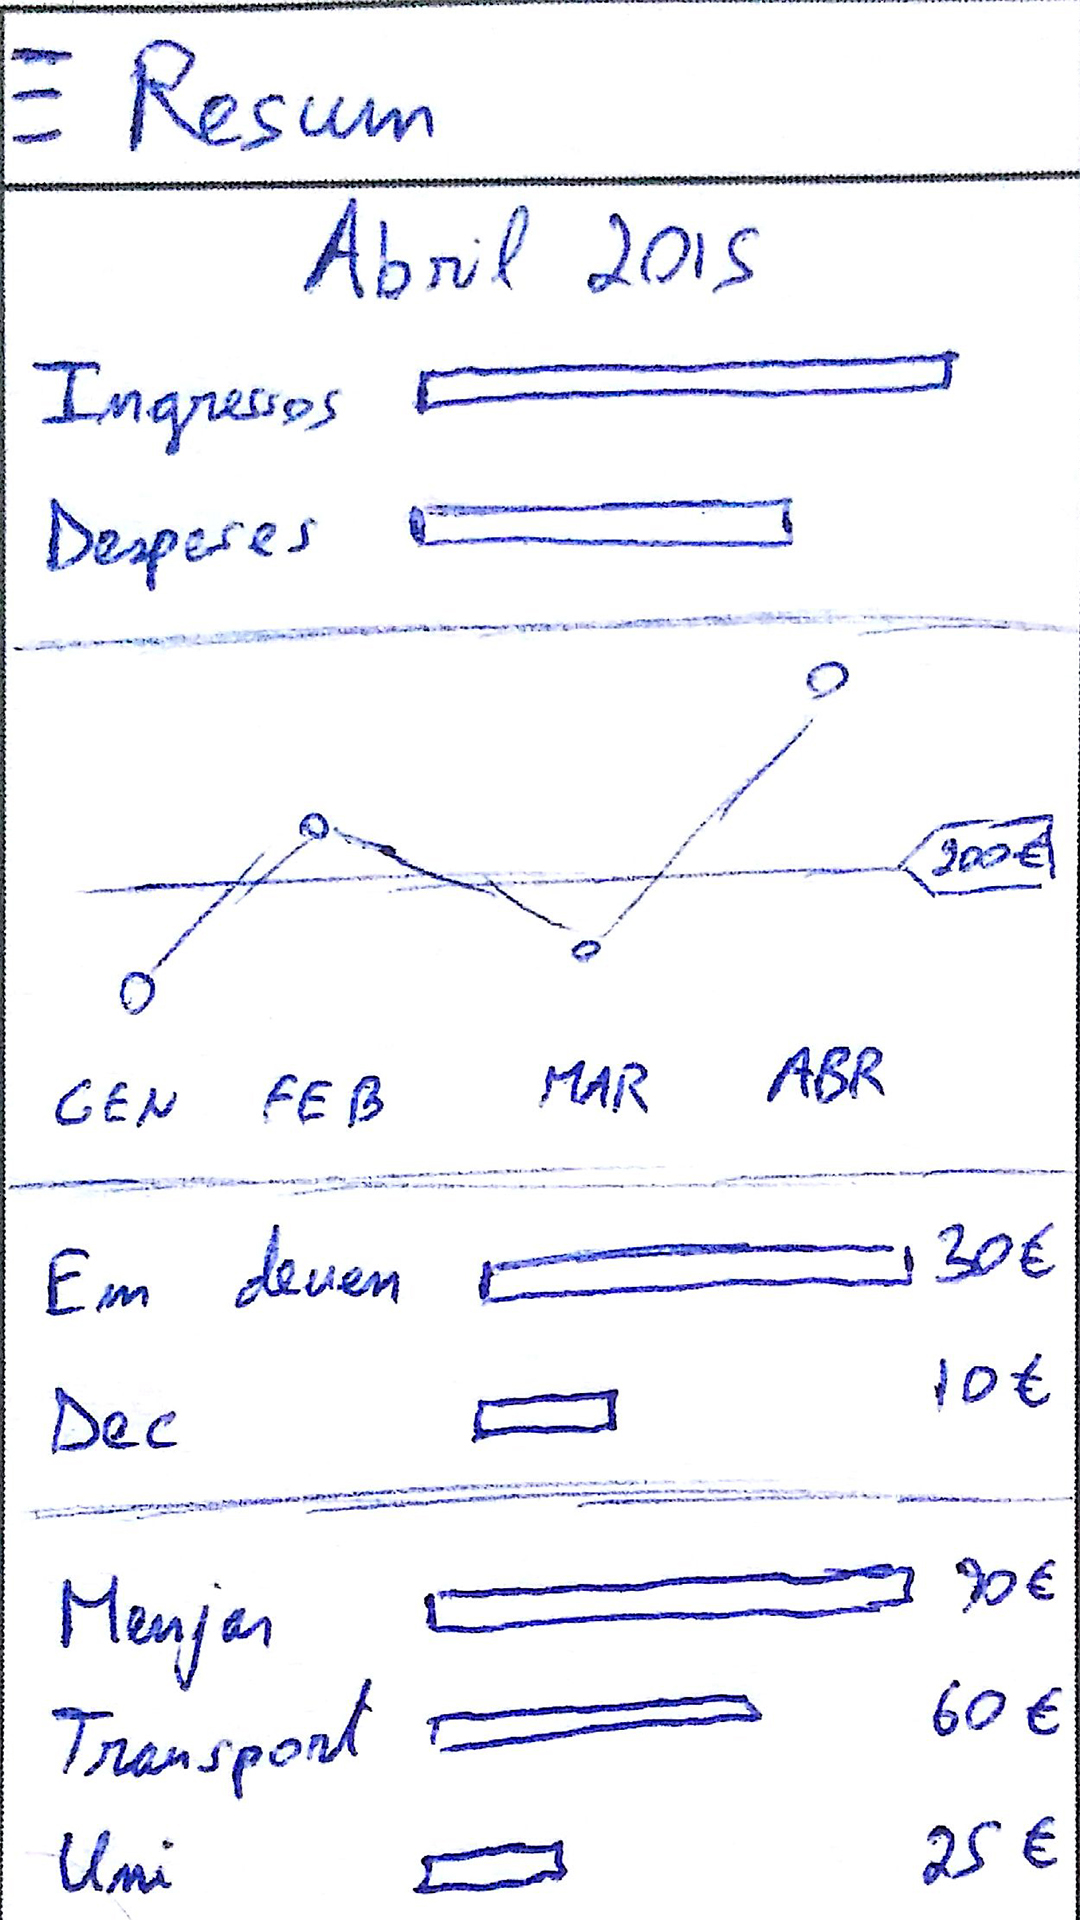
\includegraphics[width=50mm]{1_Dashboard.jpg} &
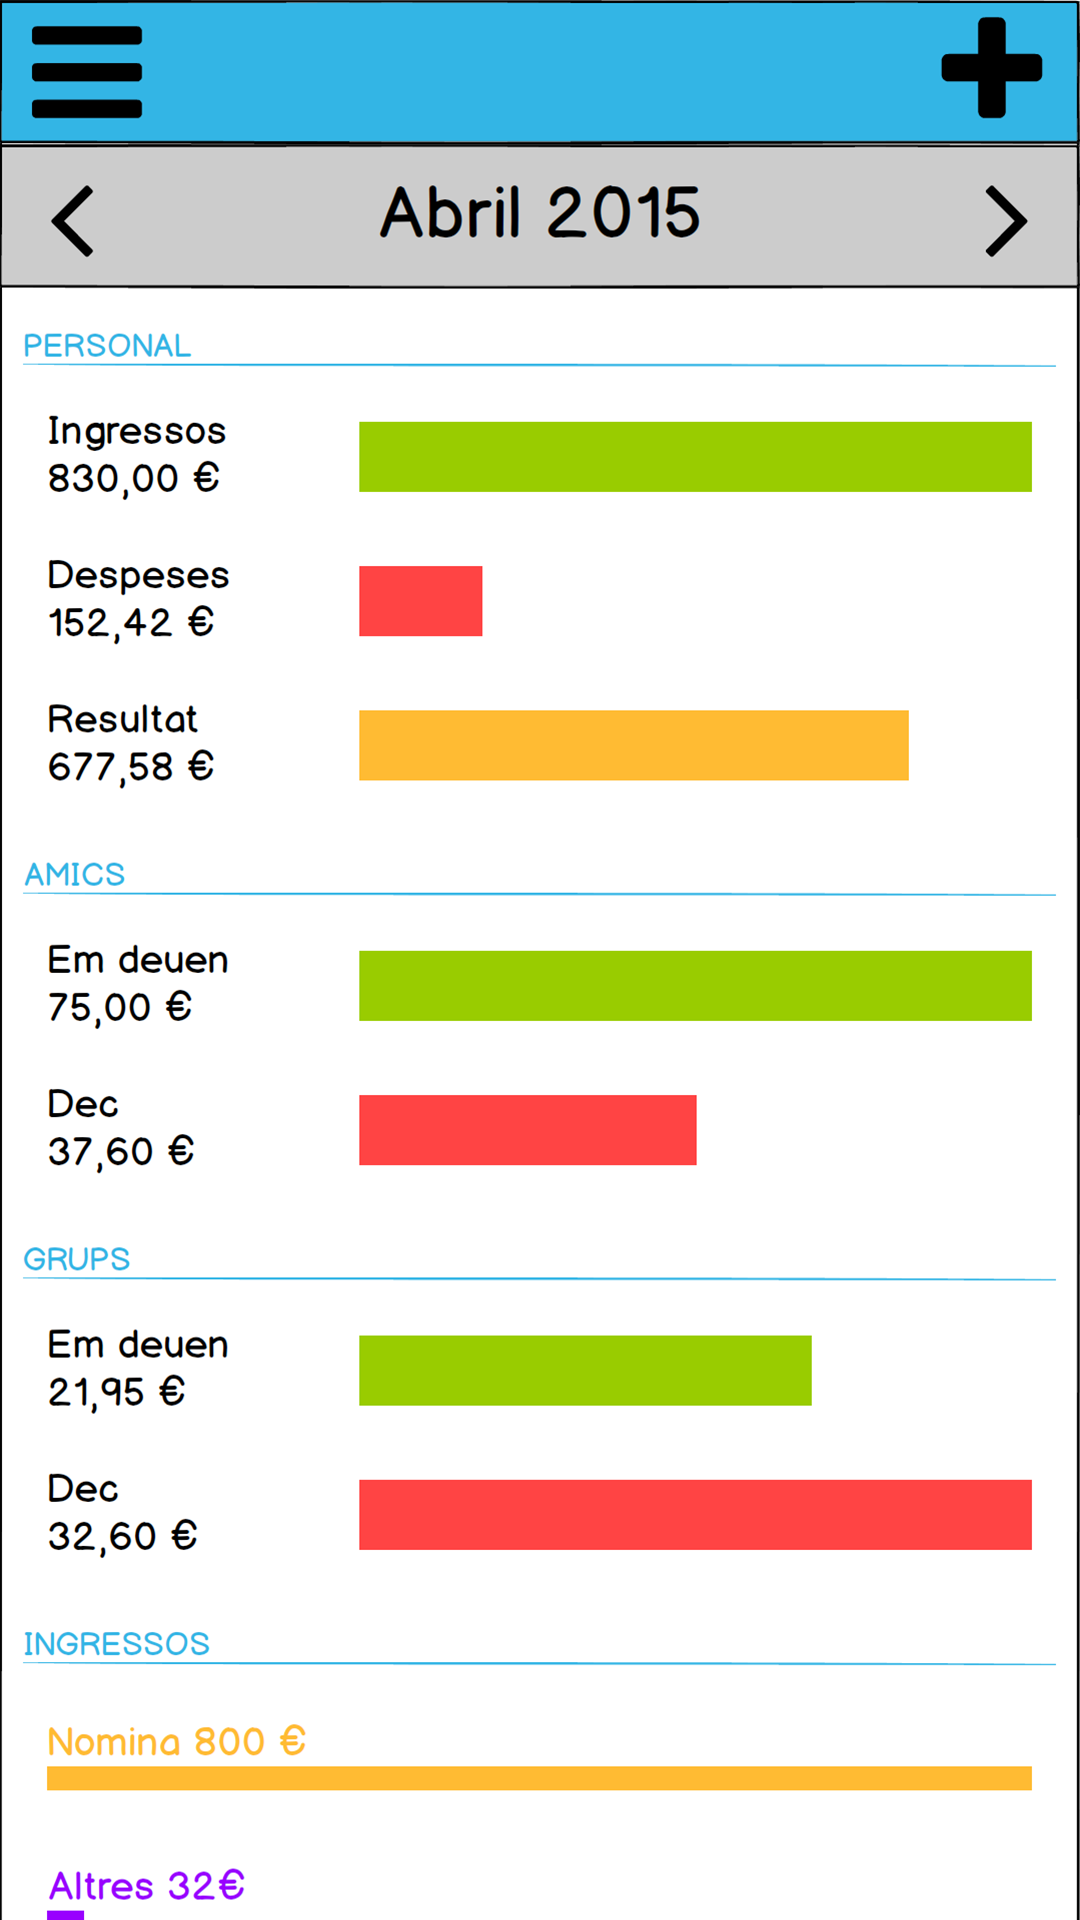
\includegraphics[width=50mm]{2_Dashboard.png} &
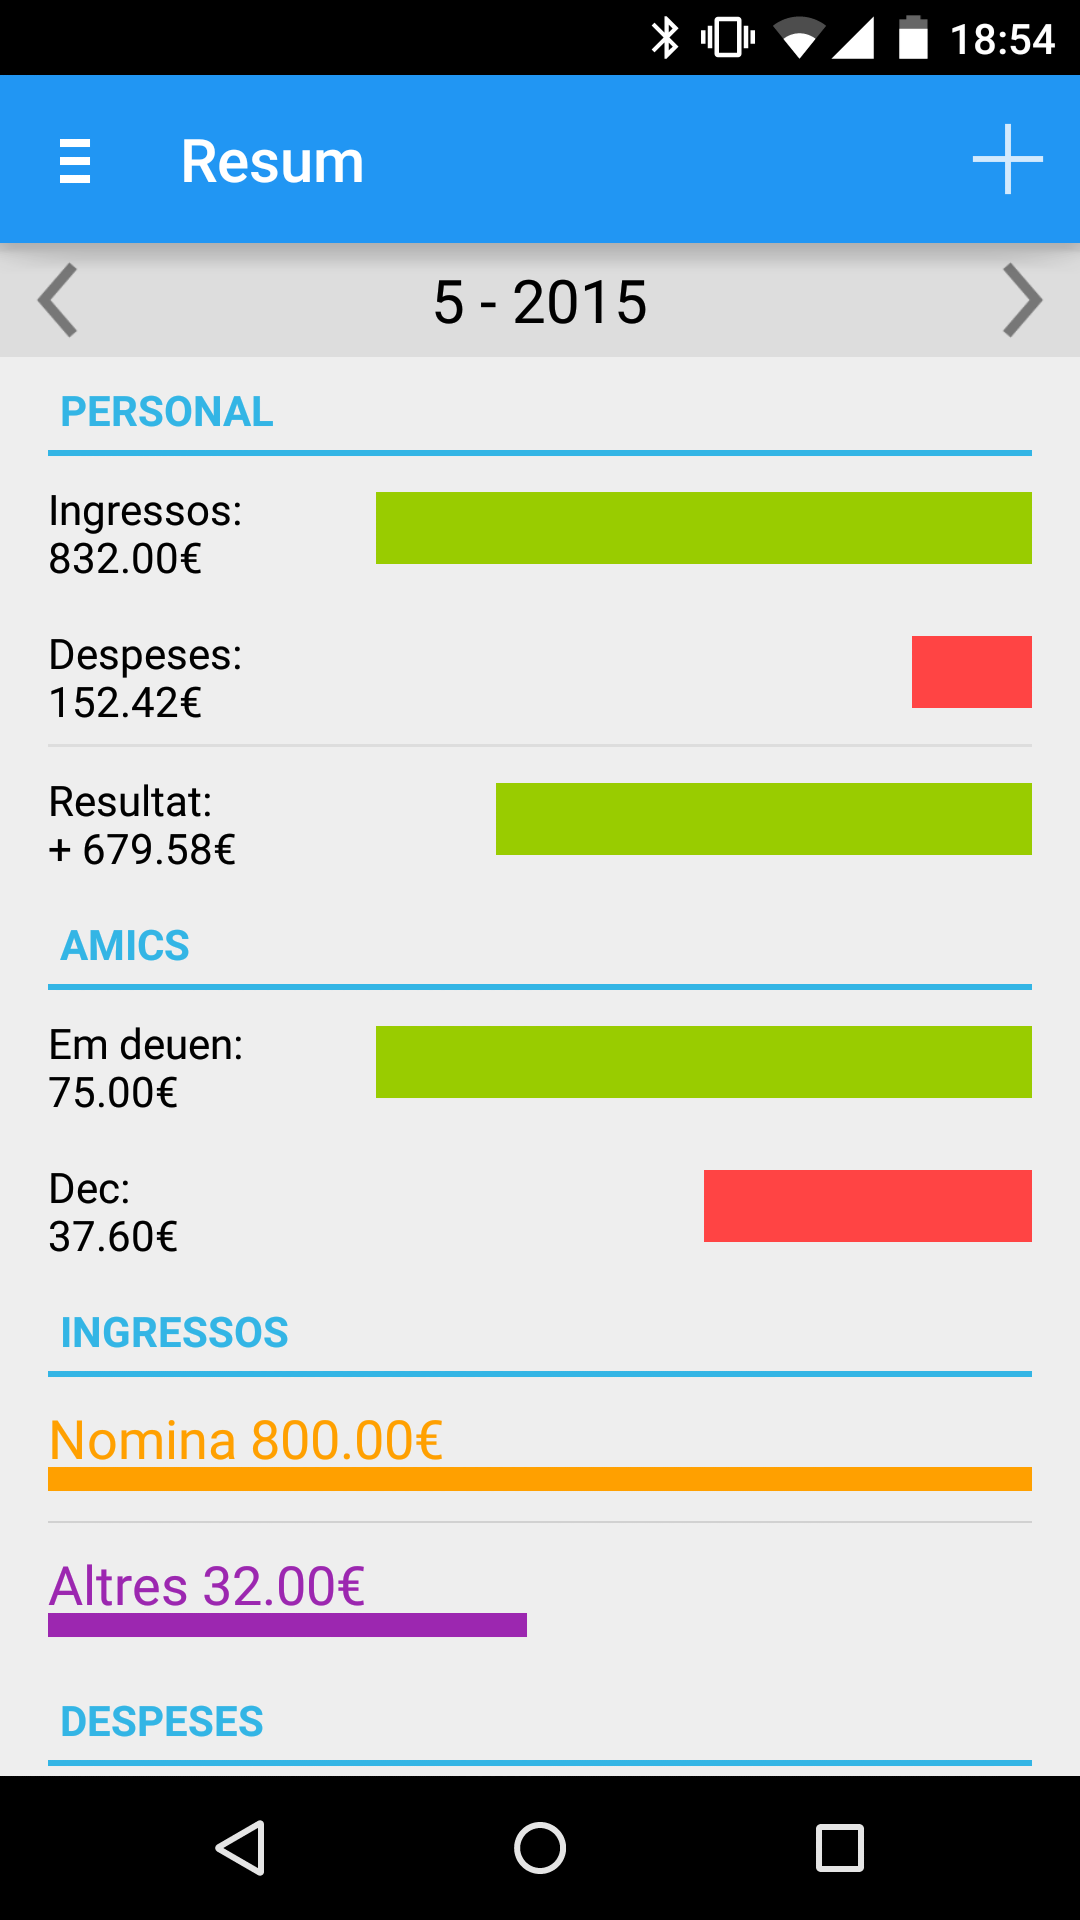
\includegraphics[width=50mm]{3_Dashboard.png} \\
\hline
Esbossos & Disseny Conceptual - intermedi & Disseny detallat - refinat \\
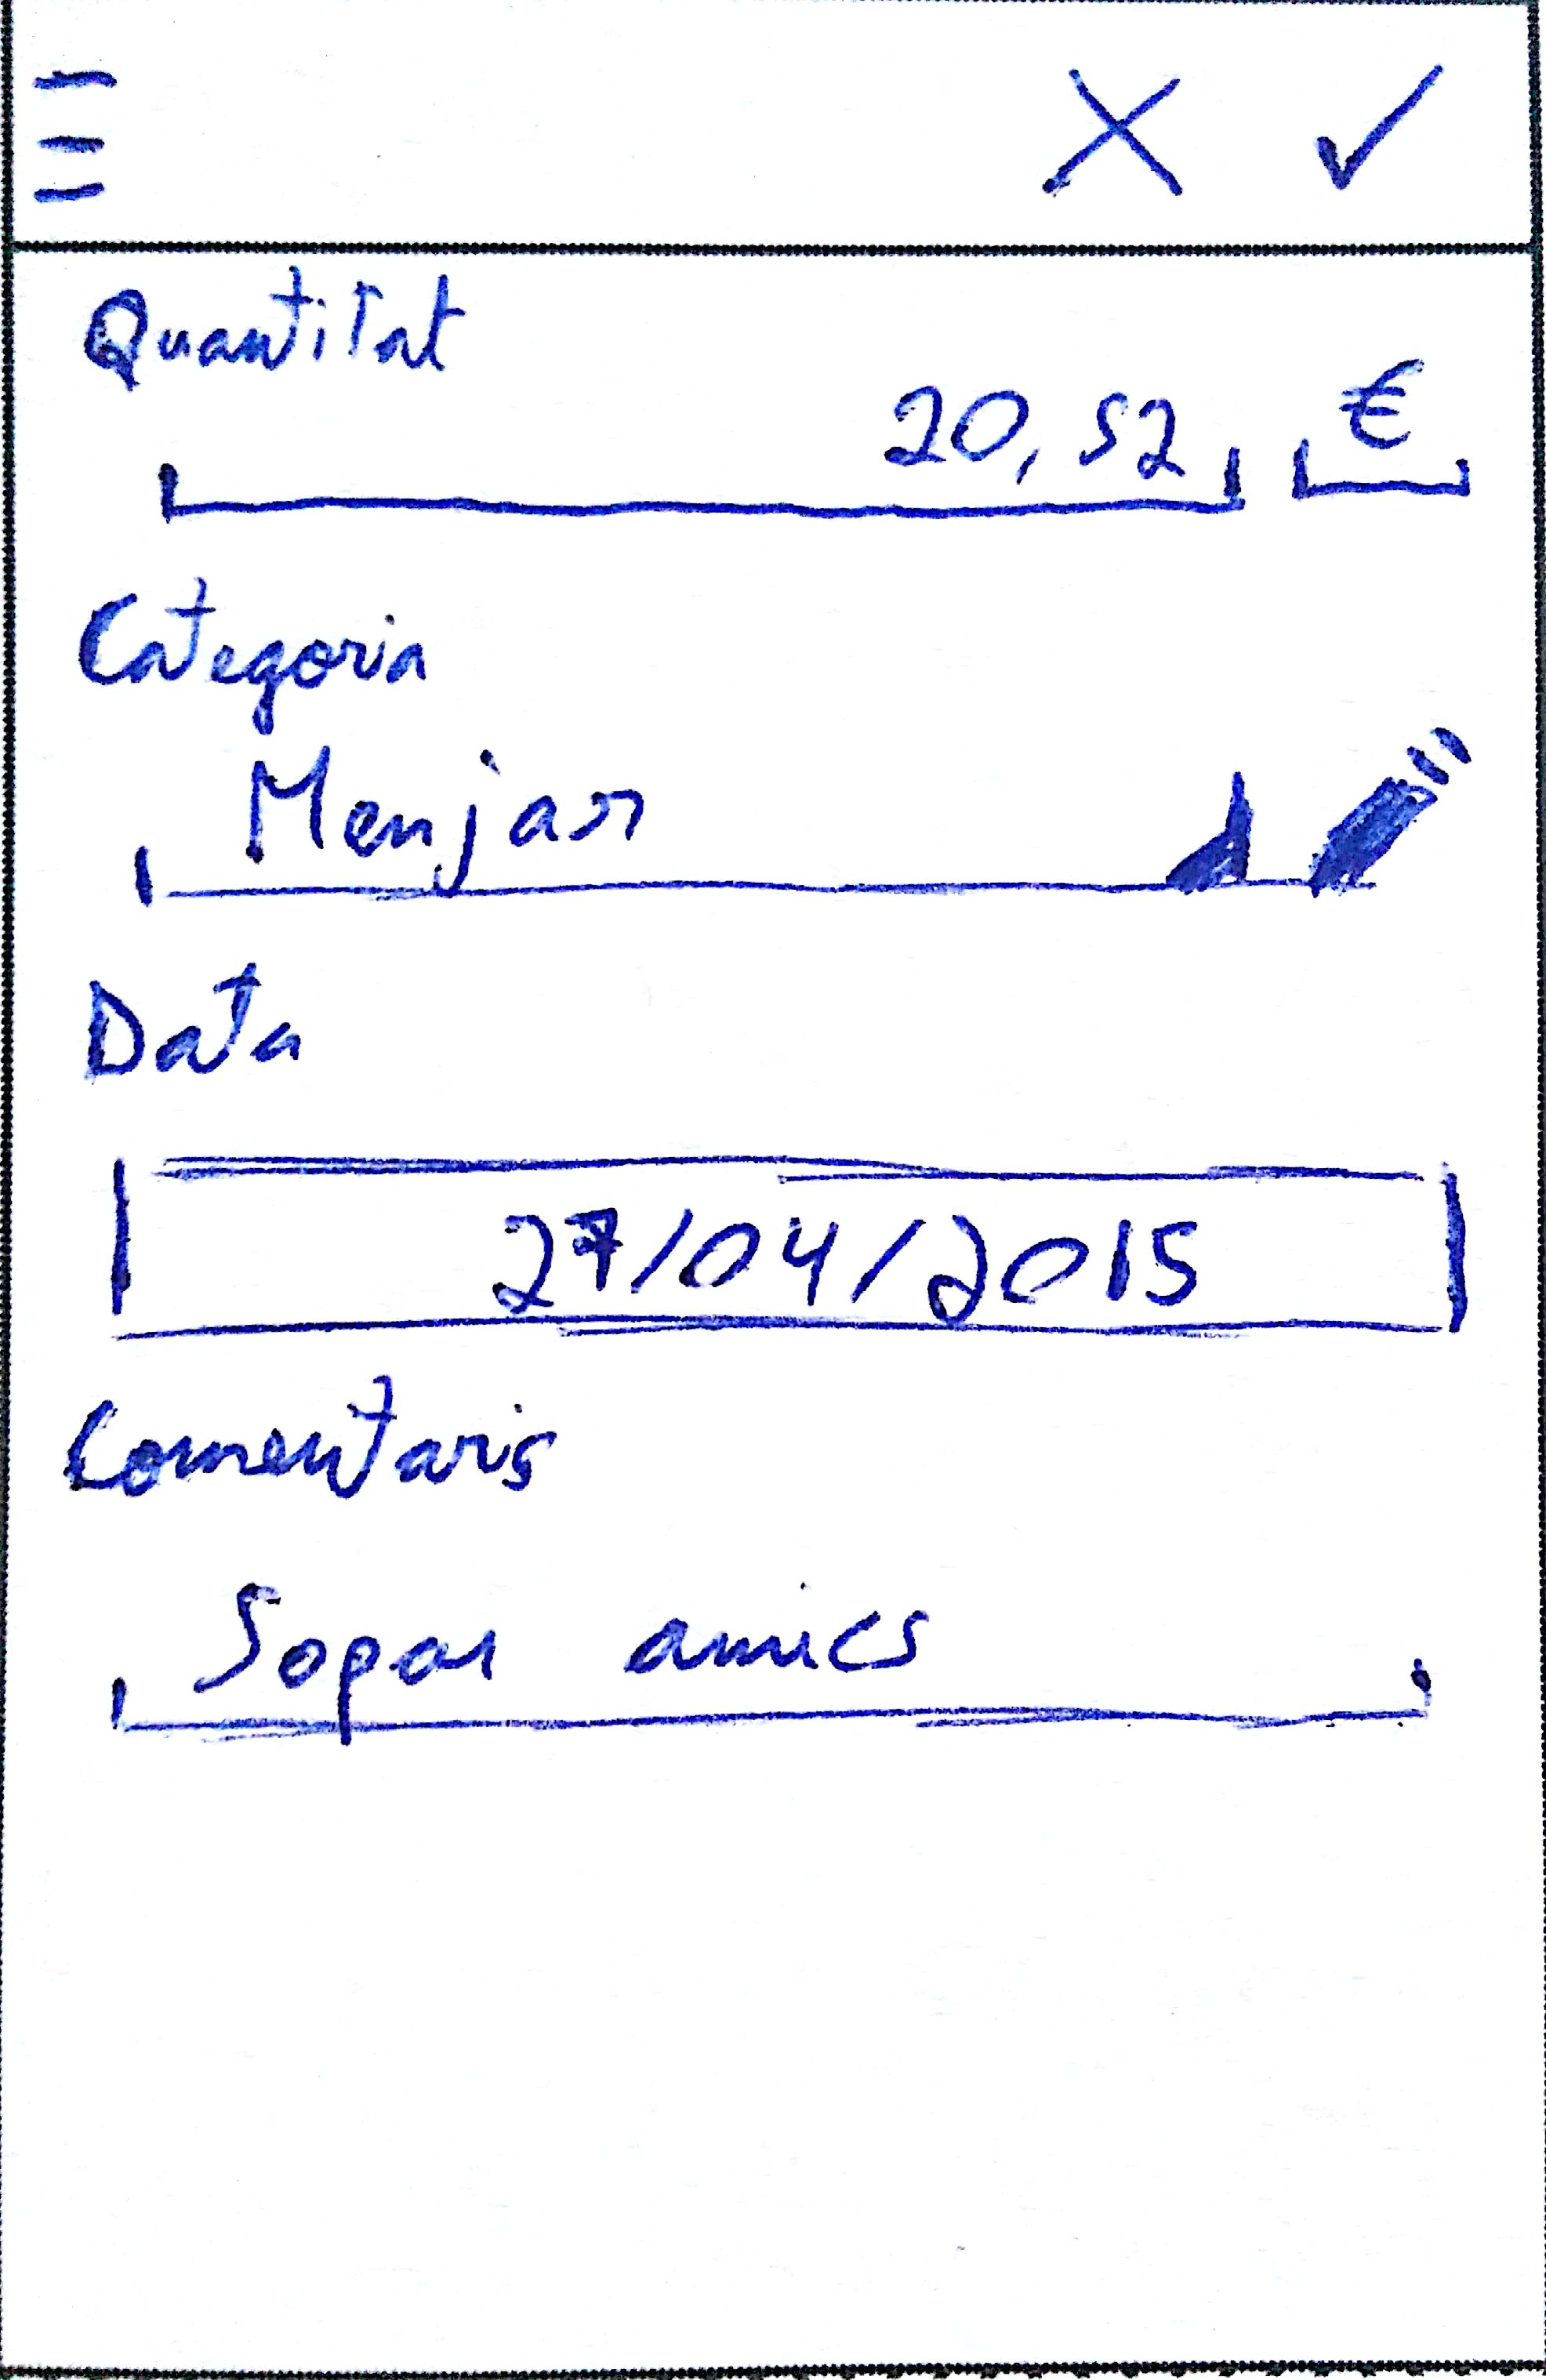
\includegraphics[width=50mm]{1_Add_expense.jpg} &
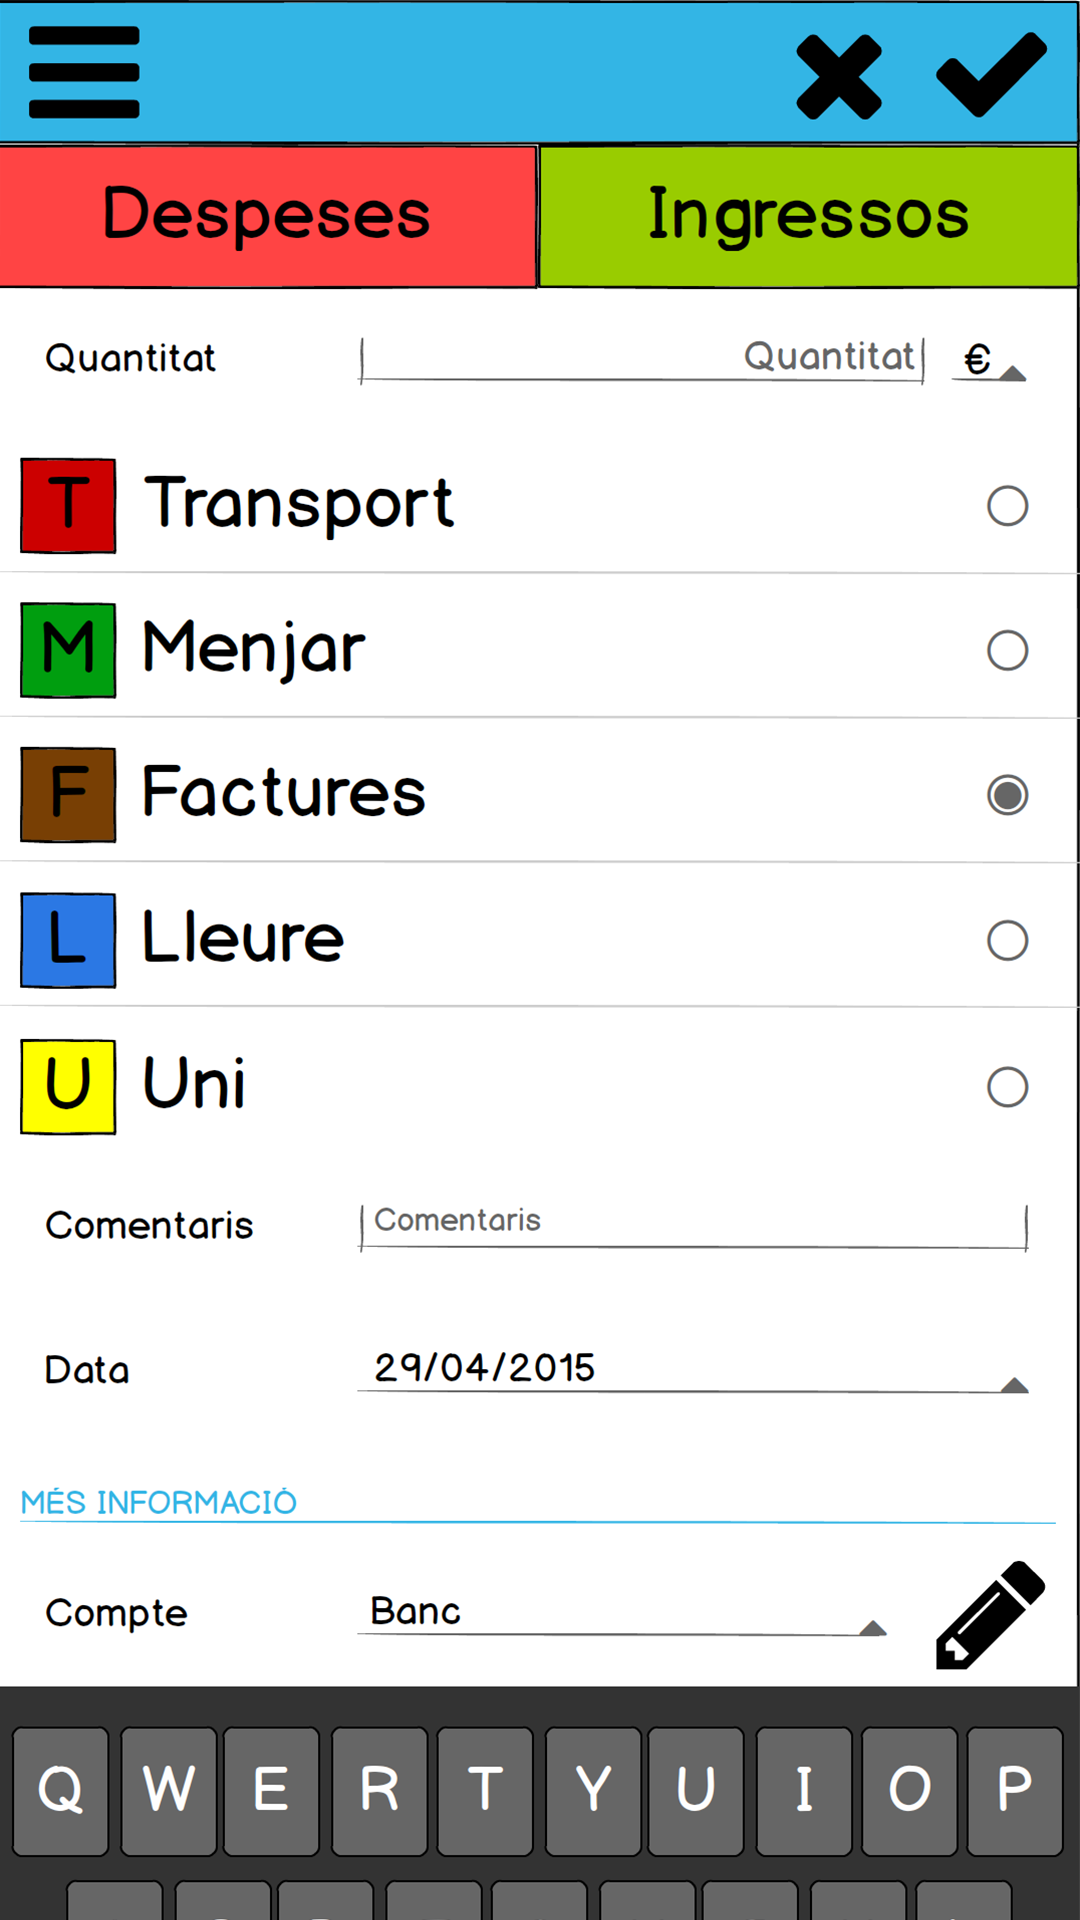
\includegraphics[width=50mm]{2_Add_expense.png} &
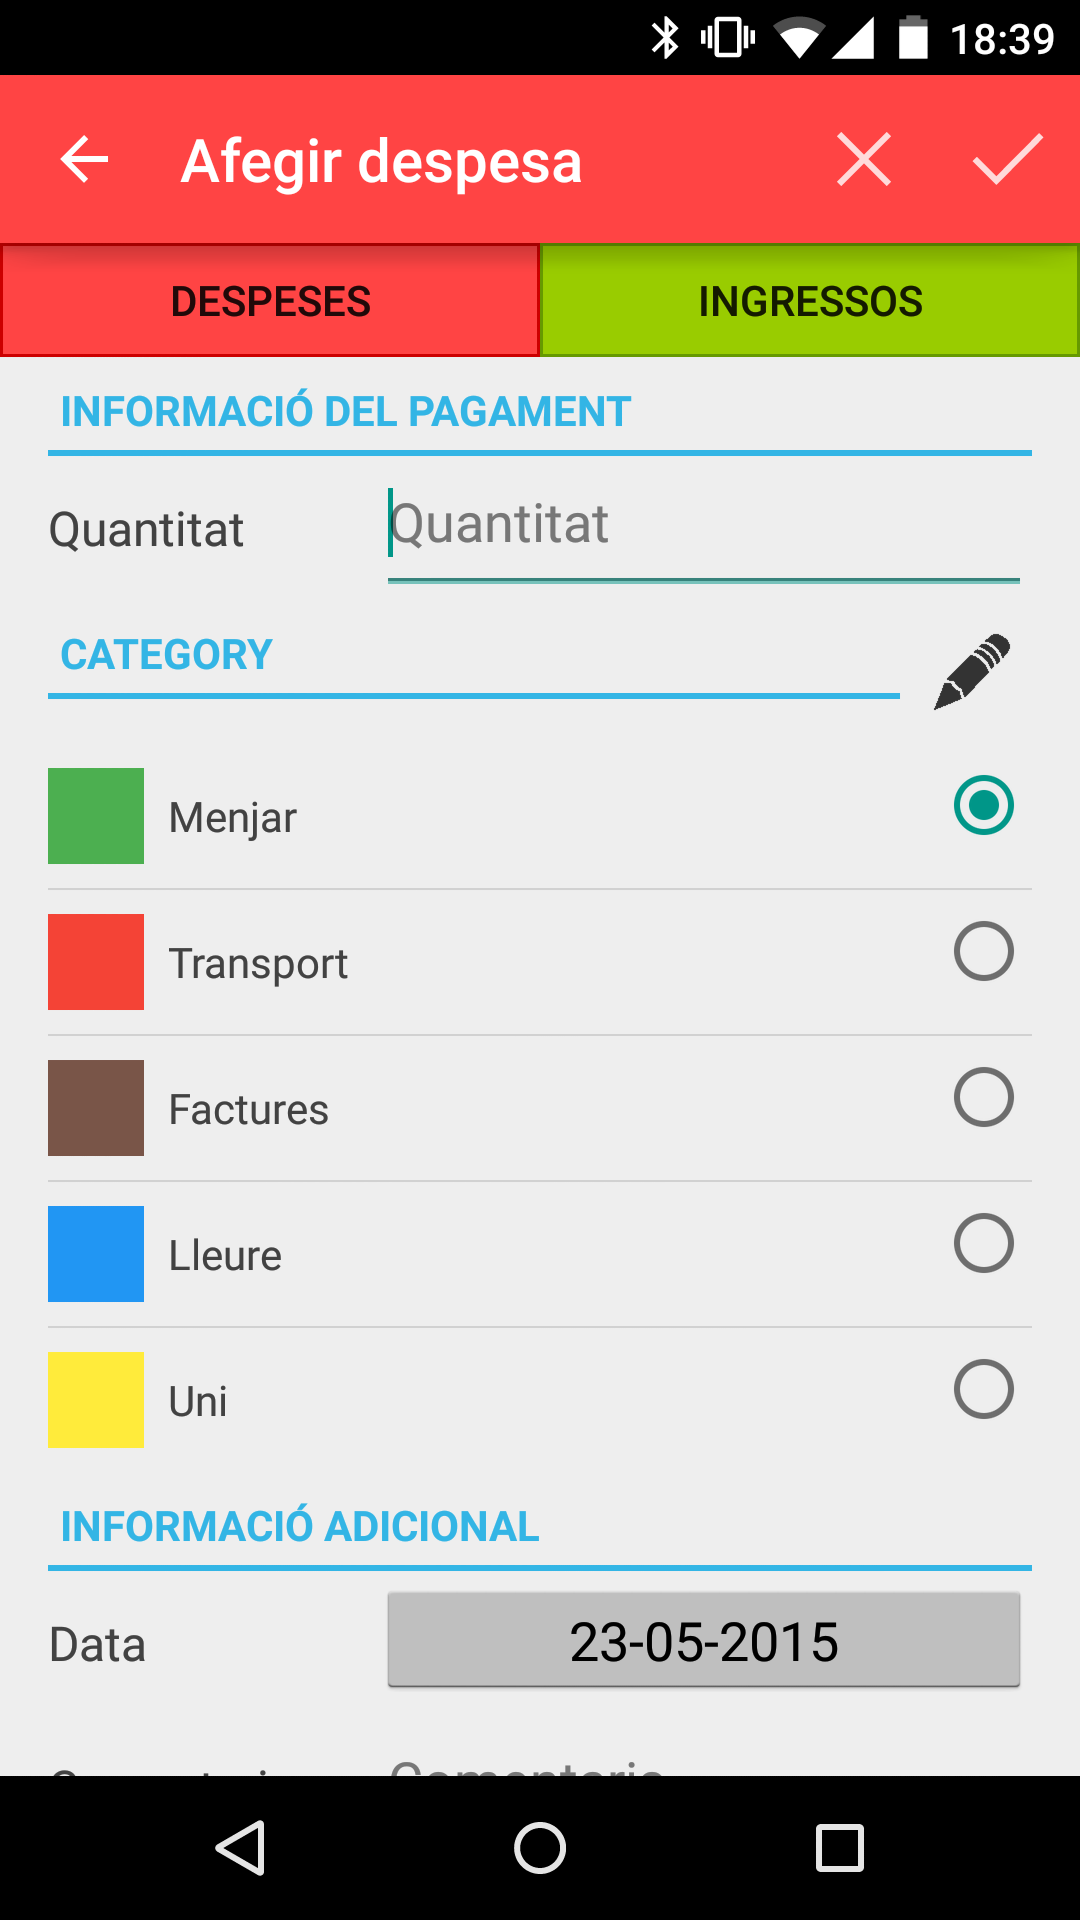
\includegraphics[width=50mm]{3_Add_expense.png} \\
\hline
\end{tabular}
\end{table}

\begin{table}
\caption{Imatges de l'aplicació a les diverses etapes del disseny 2}
\label{table:images_app2}
\begin{tabular}{| c | c | c |}
\hline
Esbossos & Disseny Conceptual - intermedi & Disseny detallat - refinat \\
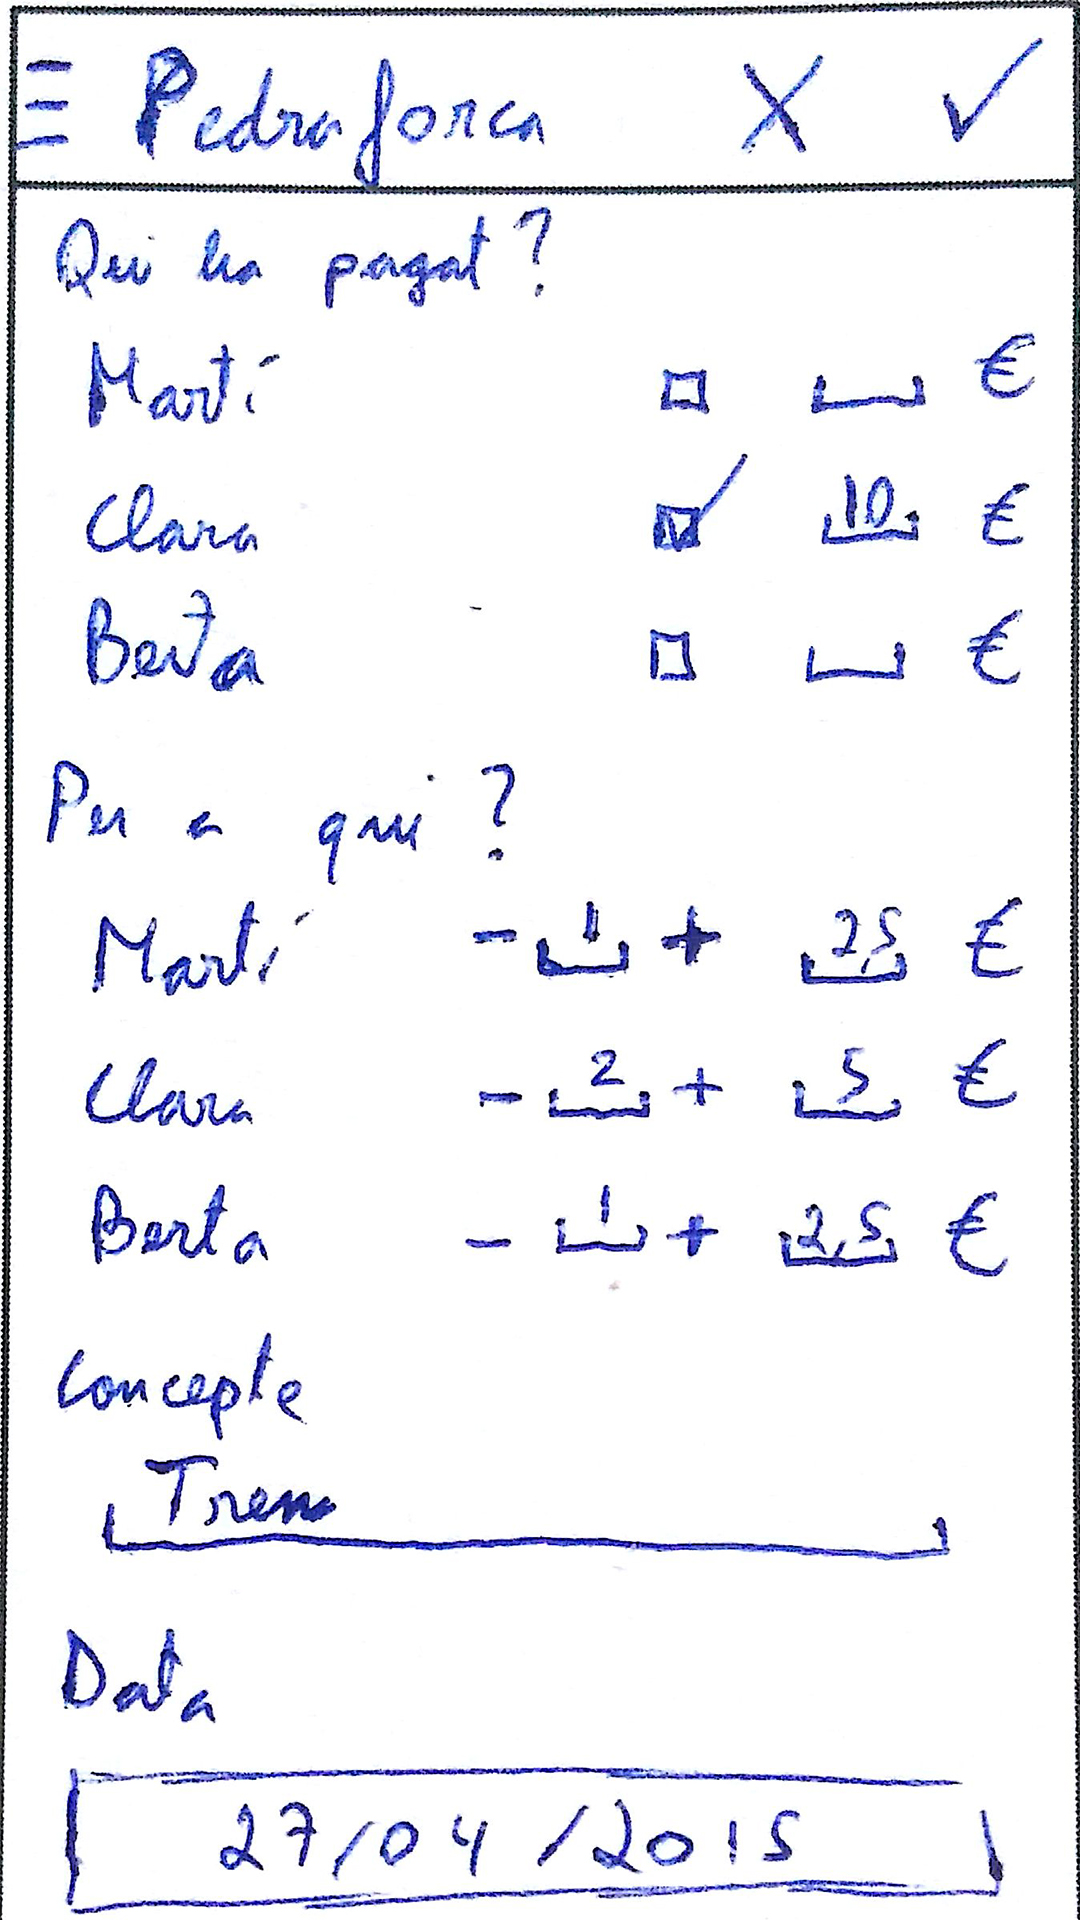
\includegraphics[width=50mm]{1_Add_group_transaction.jpg} &
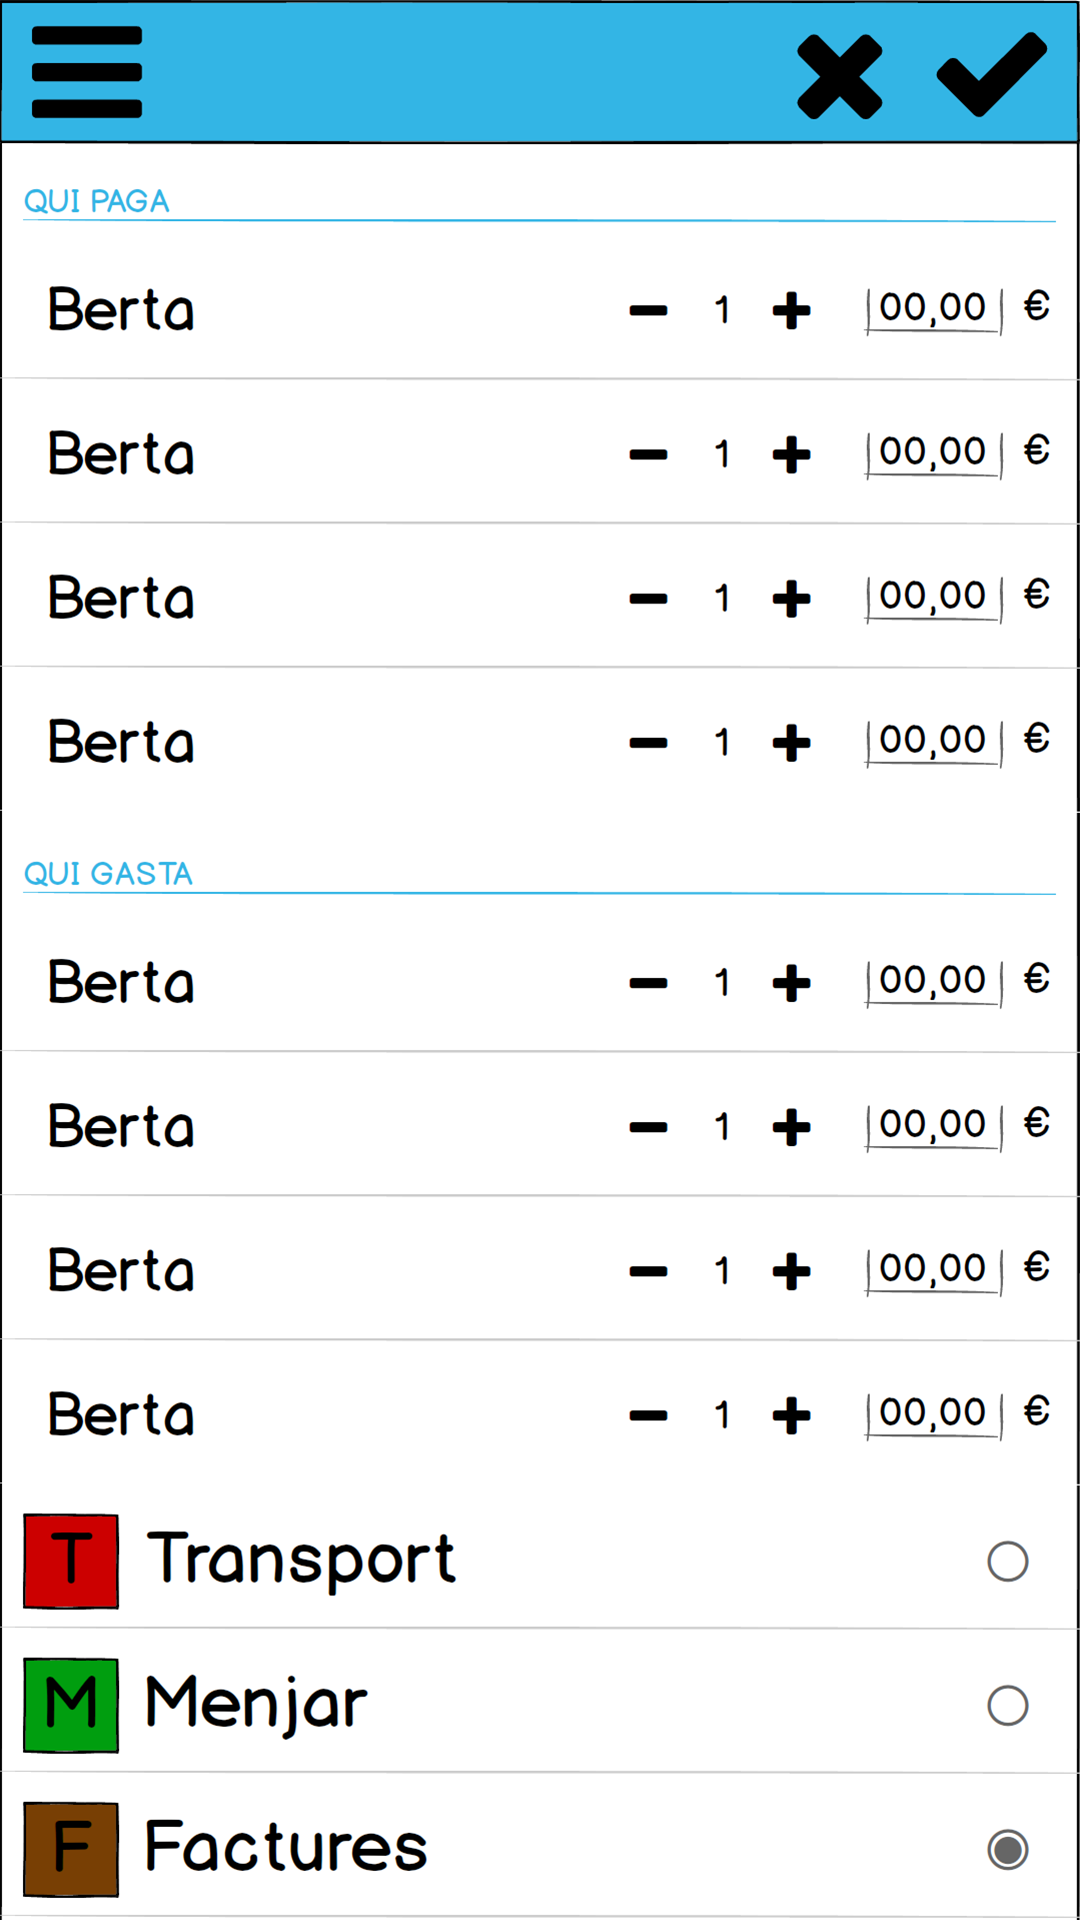
\includegraphics[width=50mm]{2_Add_group_transaction.png} &
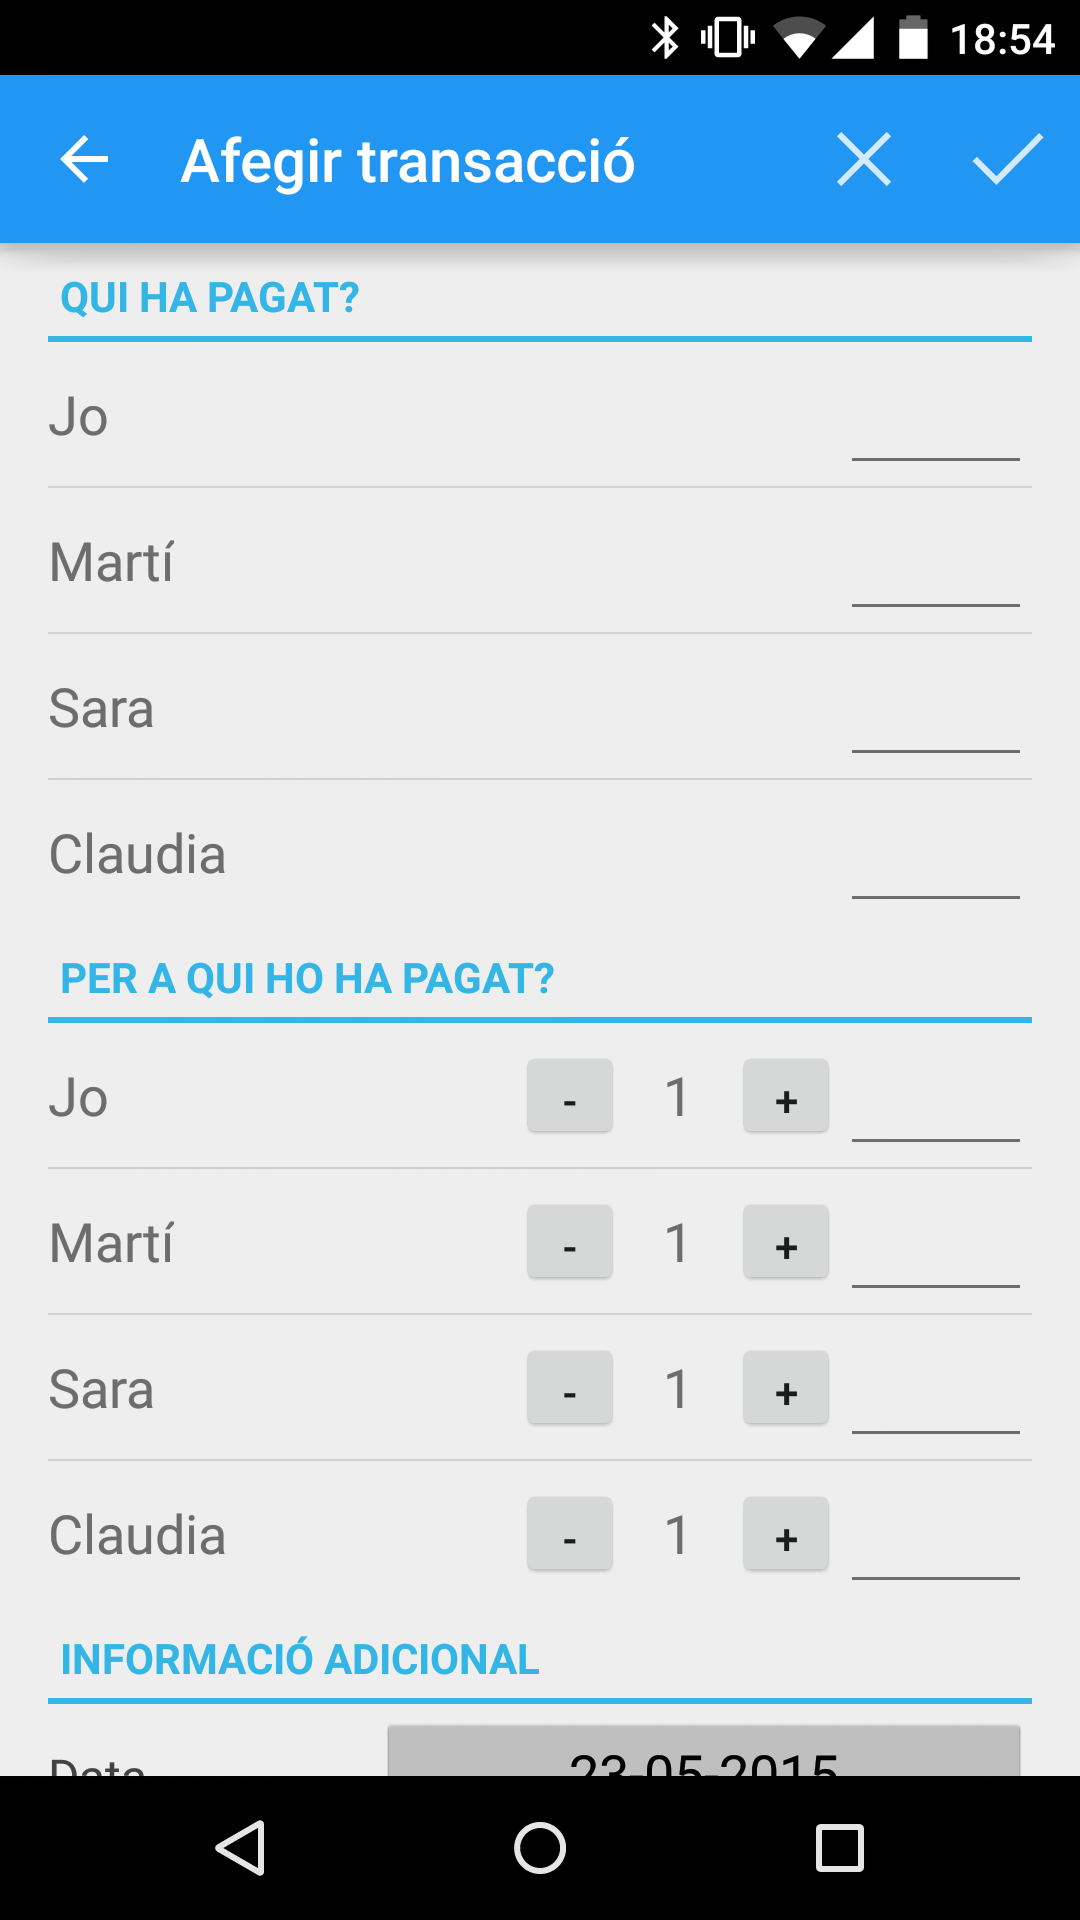
\includegraphics[width=50mm]{3_Add_group_transaction.png}  \\
\hline
Esbossos & Disseny Conceptual - intermedi & Disseny detallat - refinat \\
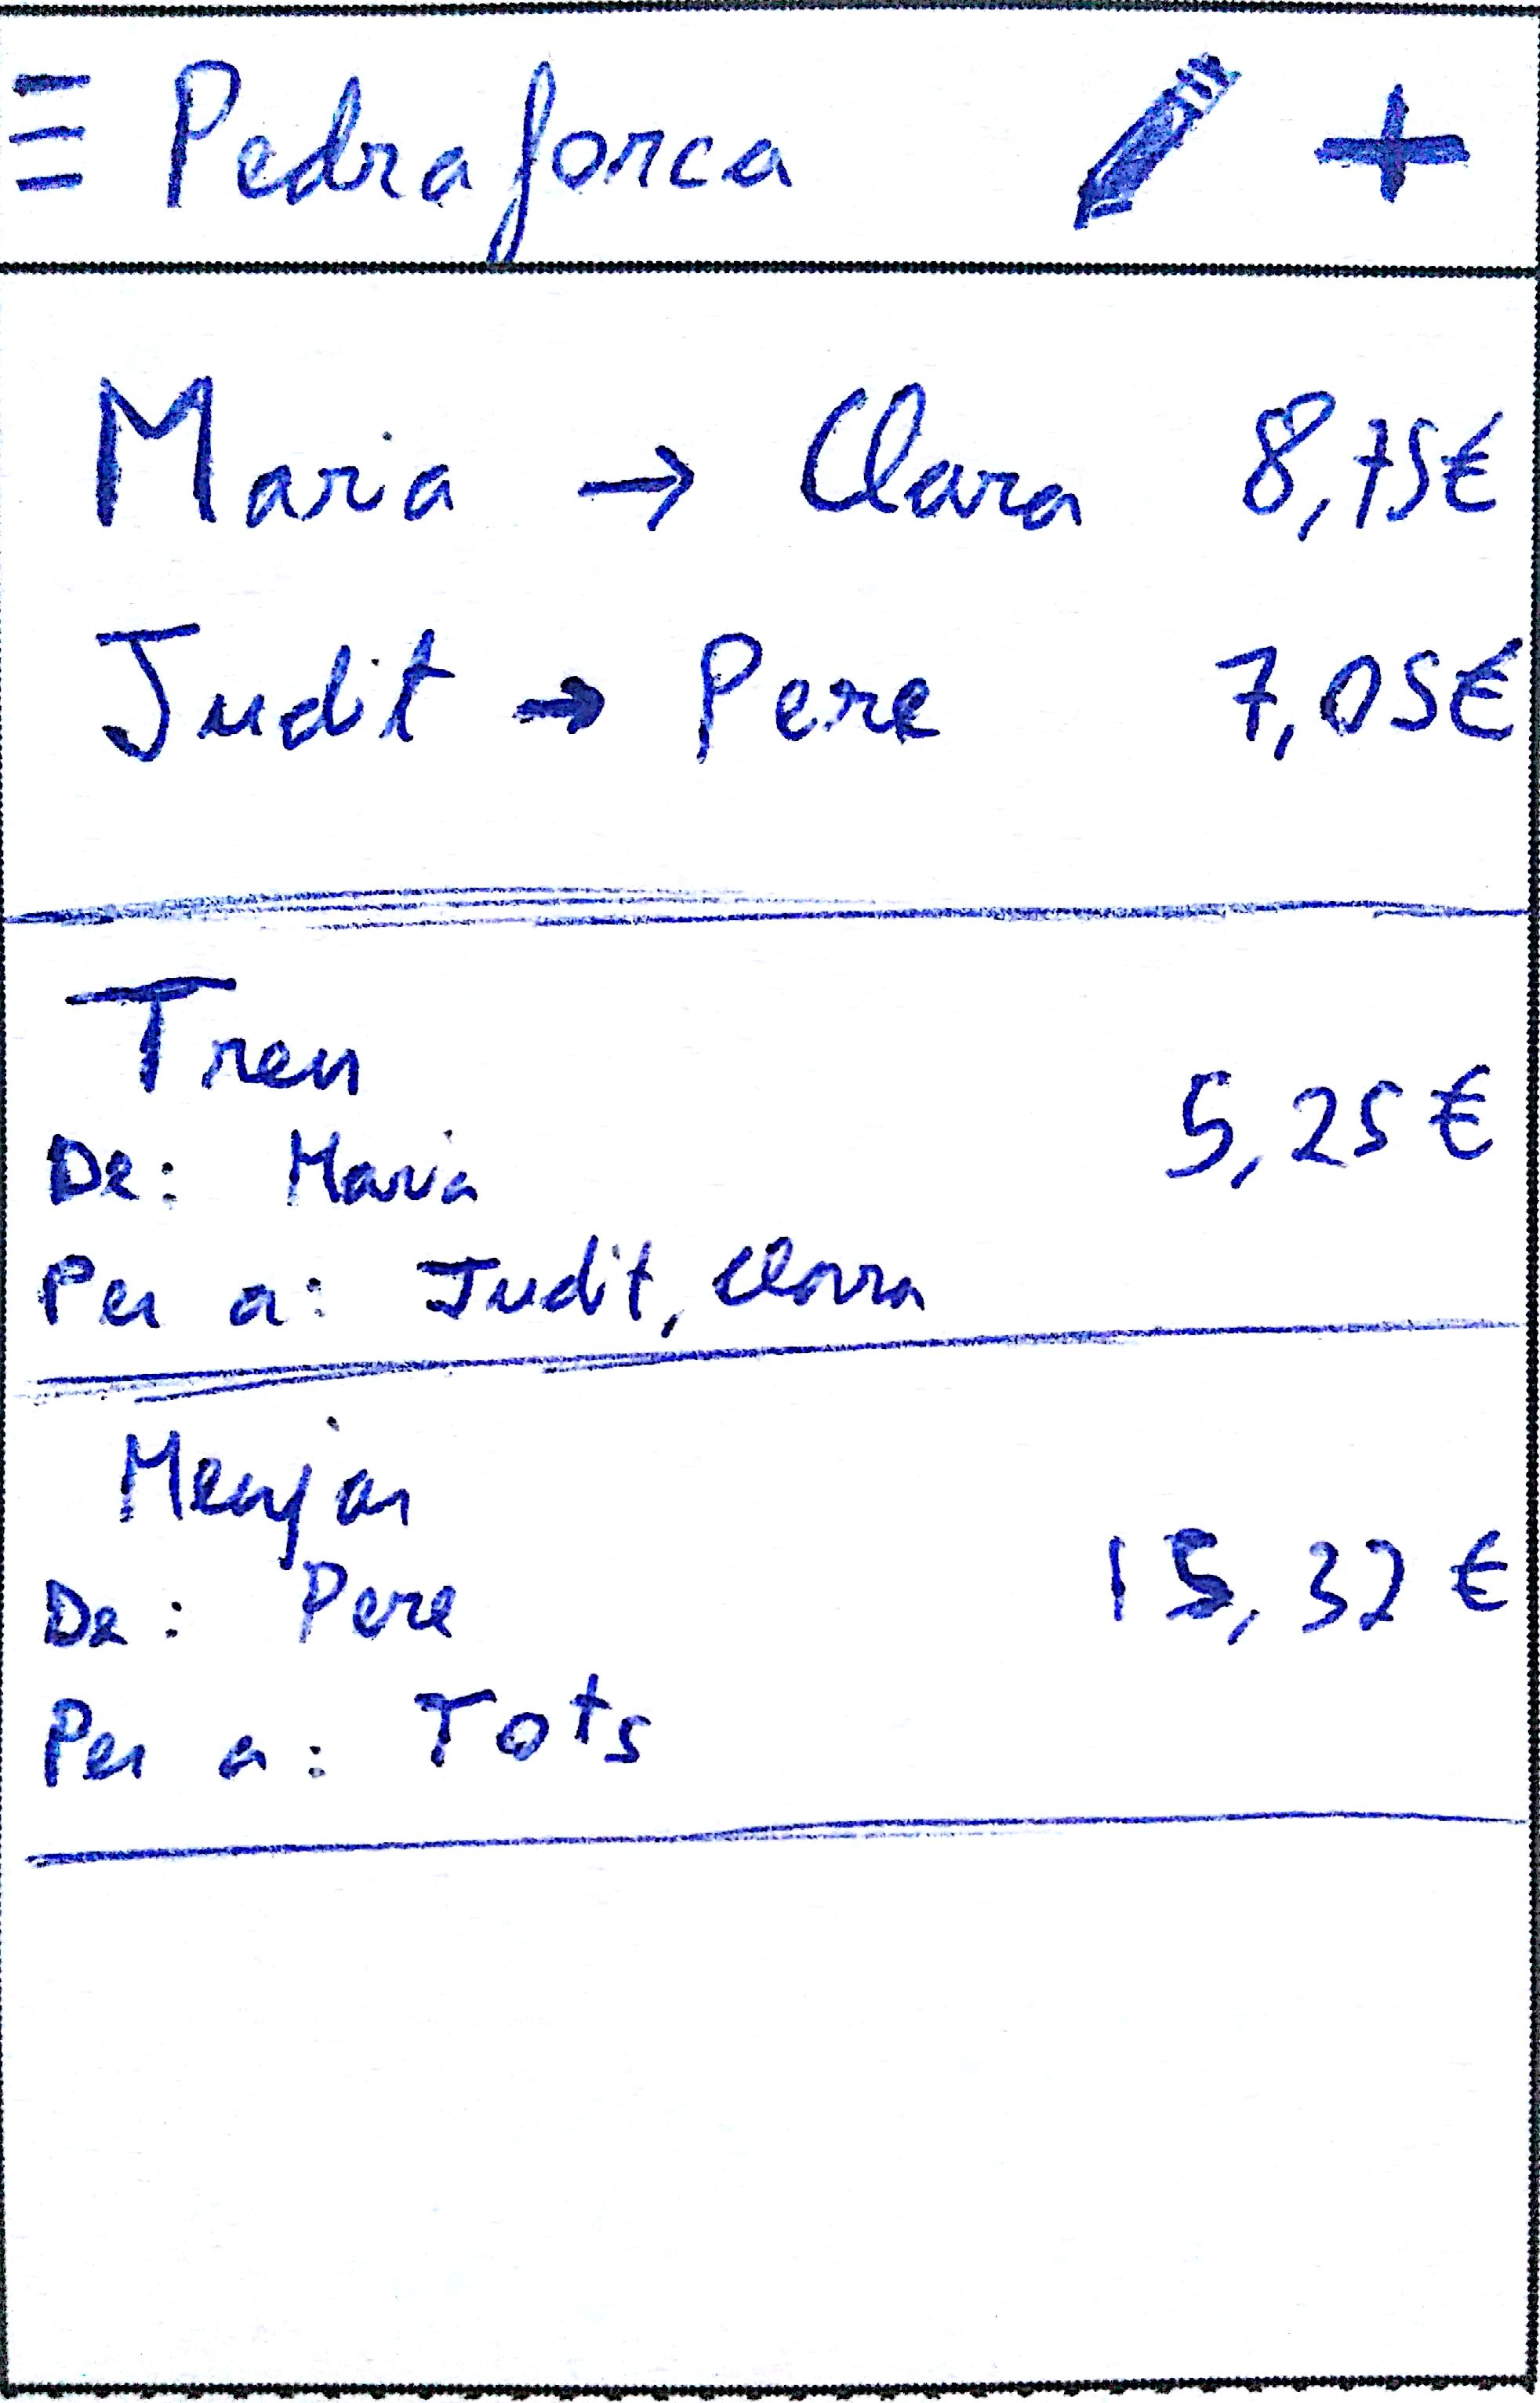
\includegraphics[width=50mm]{1_Group.jpg} &
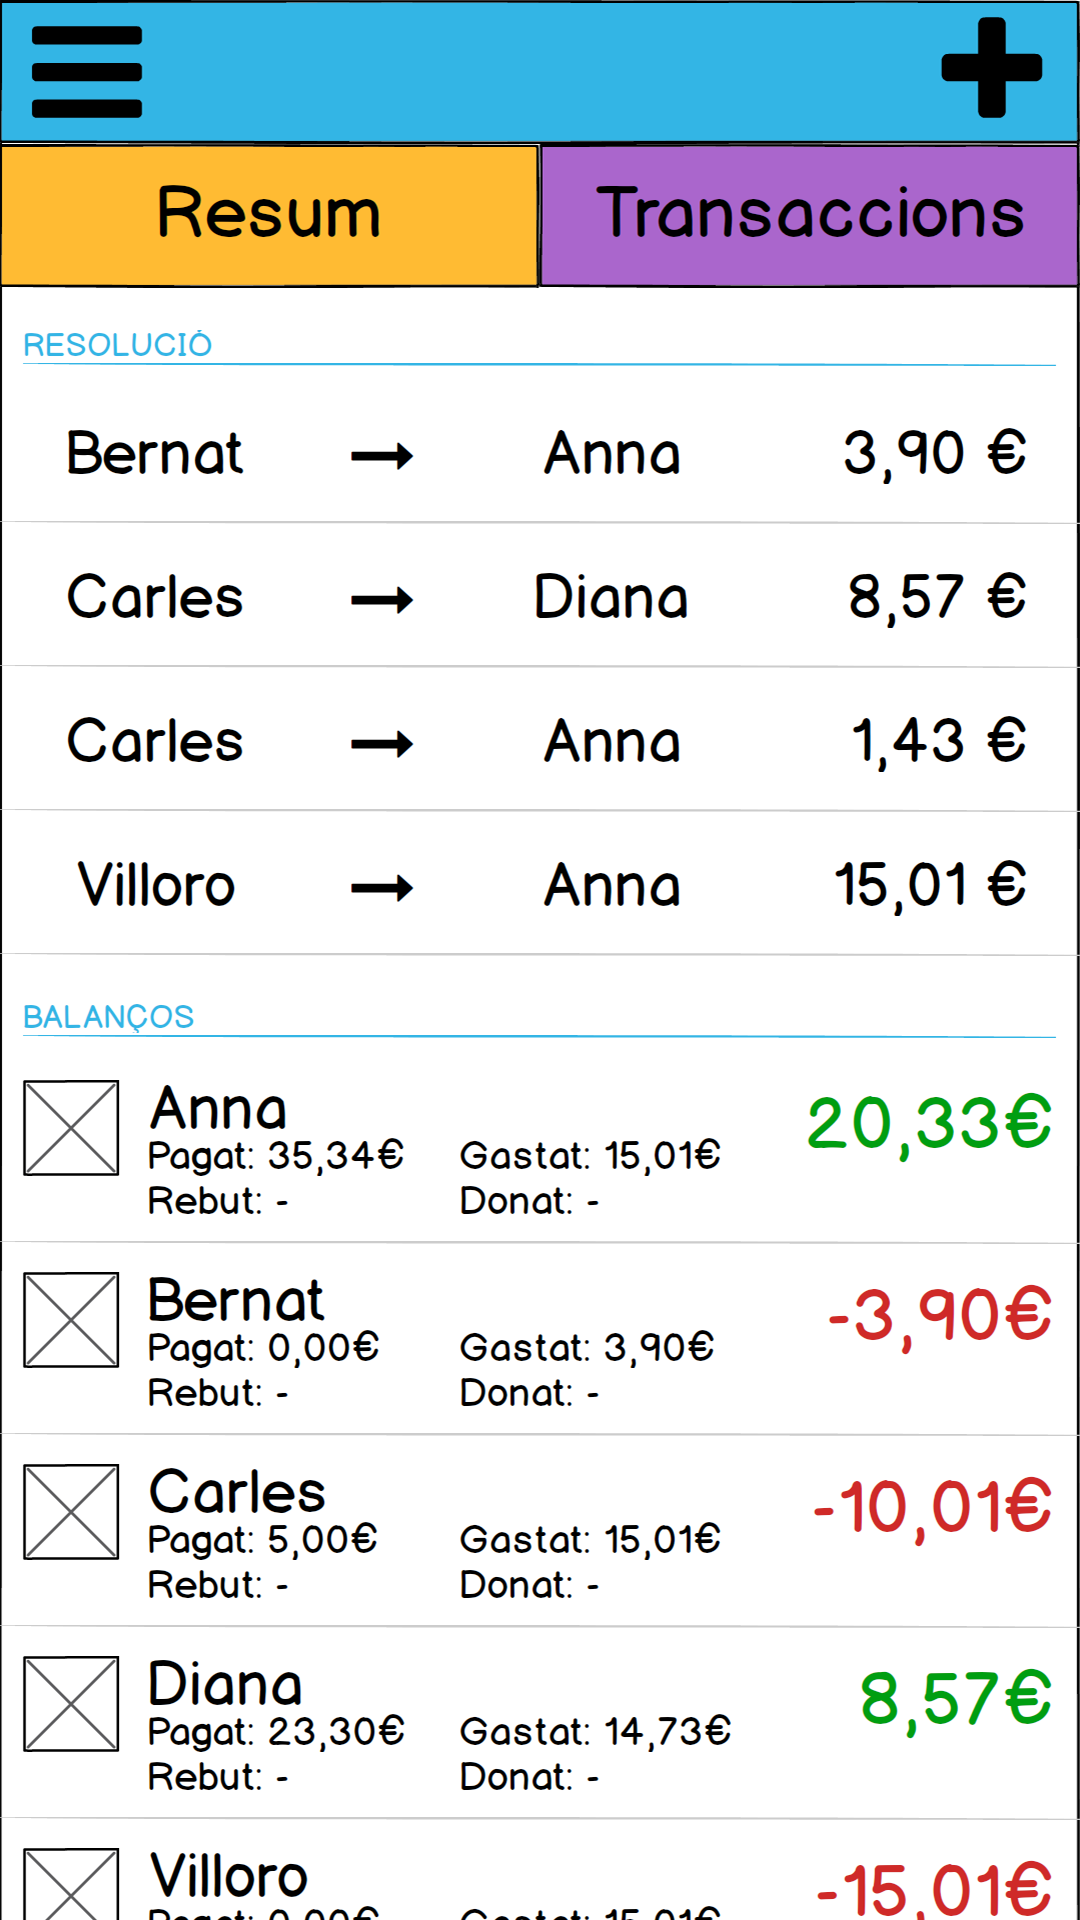
\includegraphics[width=50mm]{2_Group.png} &
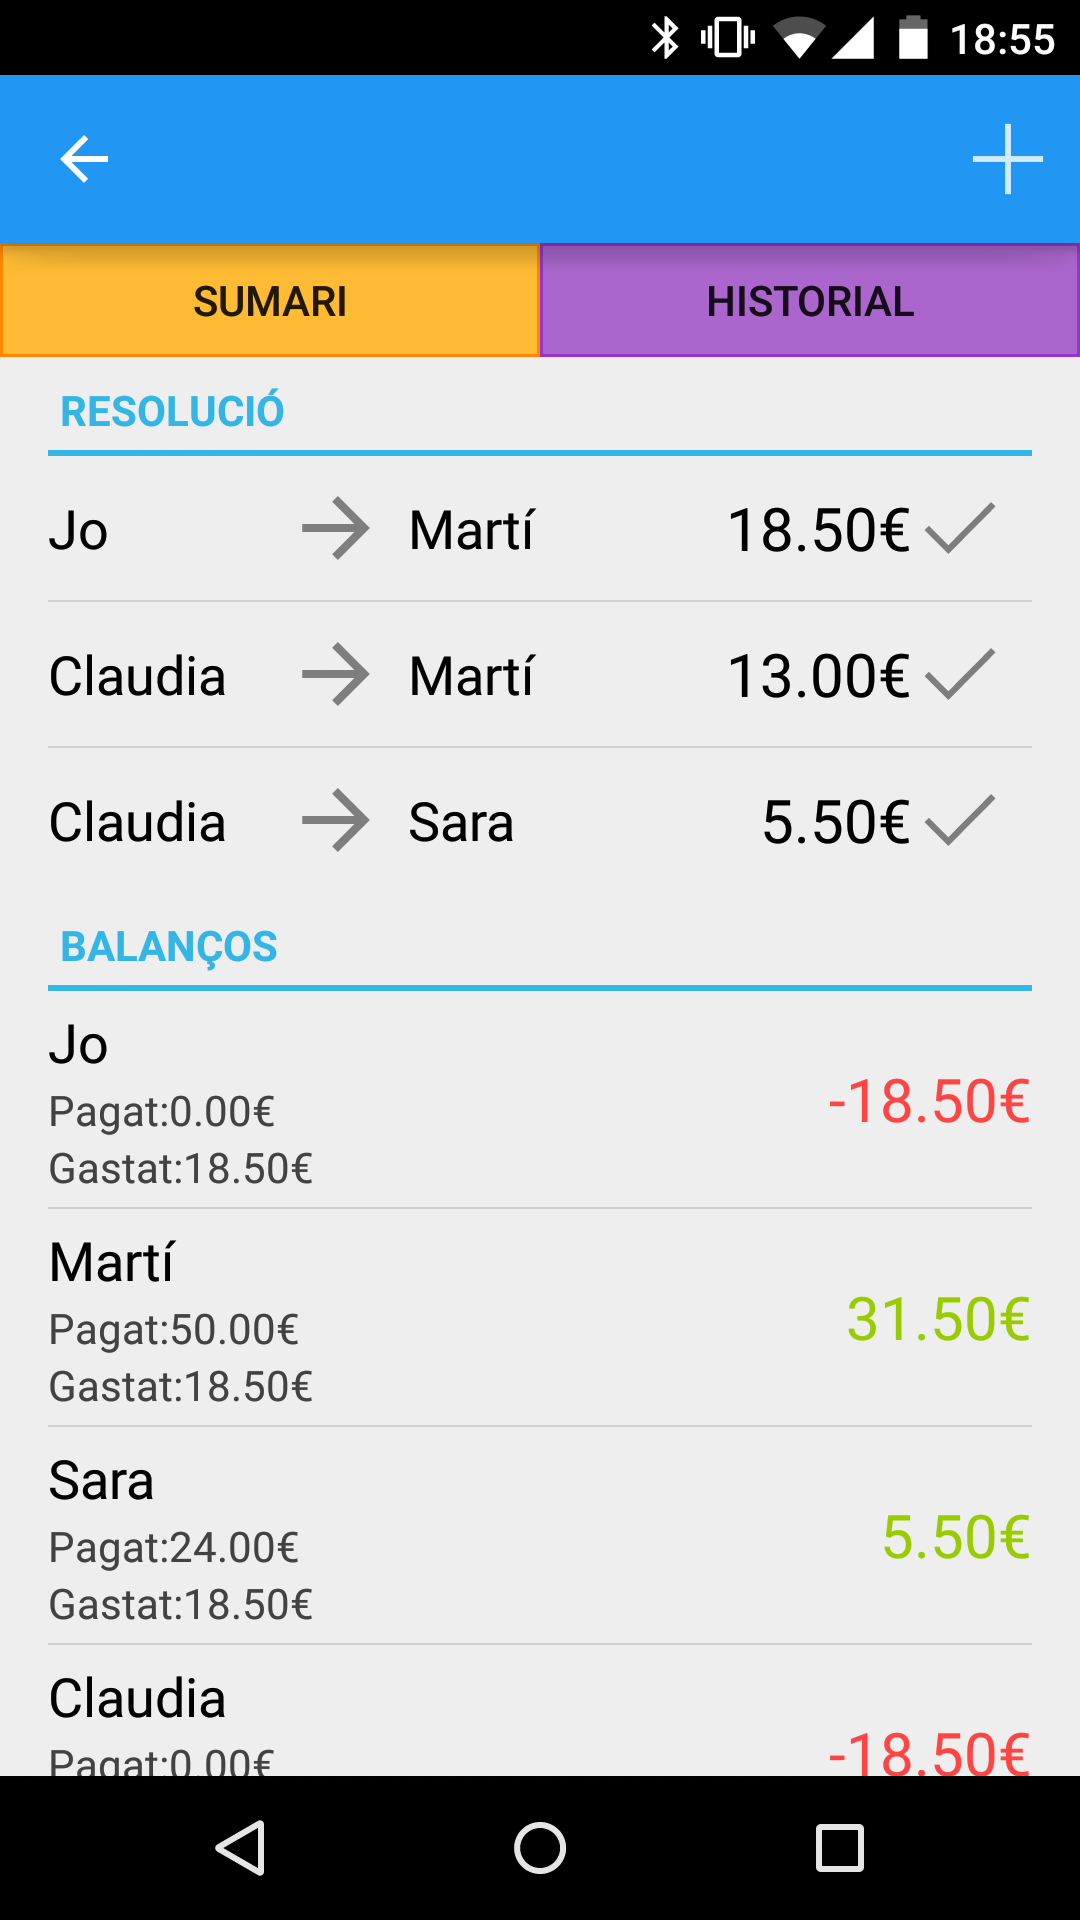
\includegraphics[width=50mm]{3_Group.png}  \\
\hline
\end{tabular}
\end{table}

\begin{table}
\caption{Imatges de l'aplicació a les diverses etapes del disseny 3}
\label{table:images_app3}
\begin{tabular}{| c | c | c |}
\hline
Esbossos & Disseny Conceptual - intermedi & Disseny detallat - refinat \\
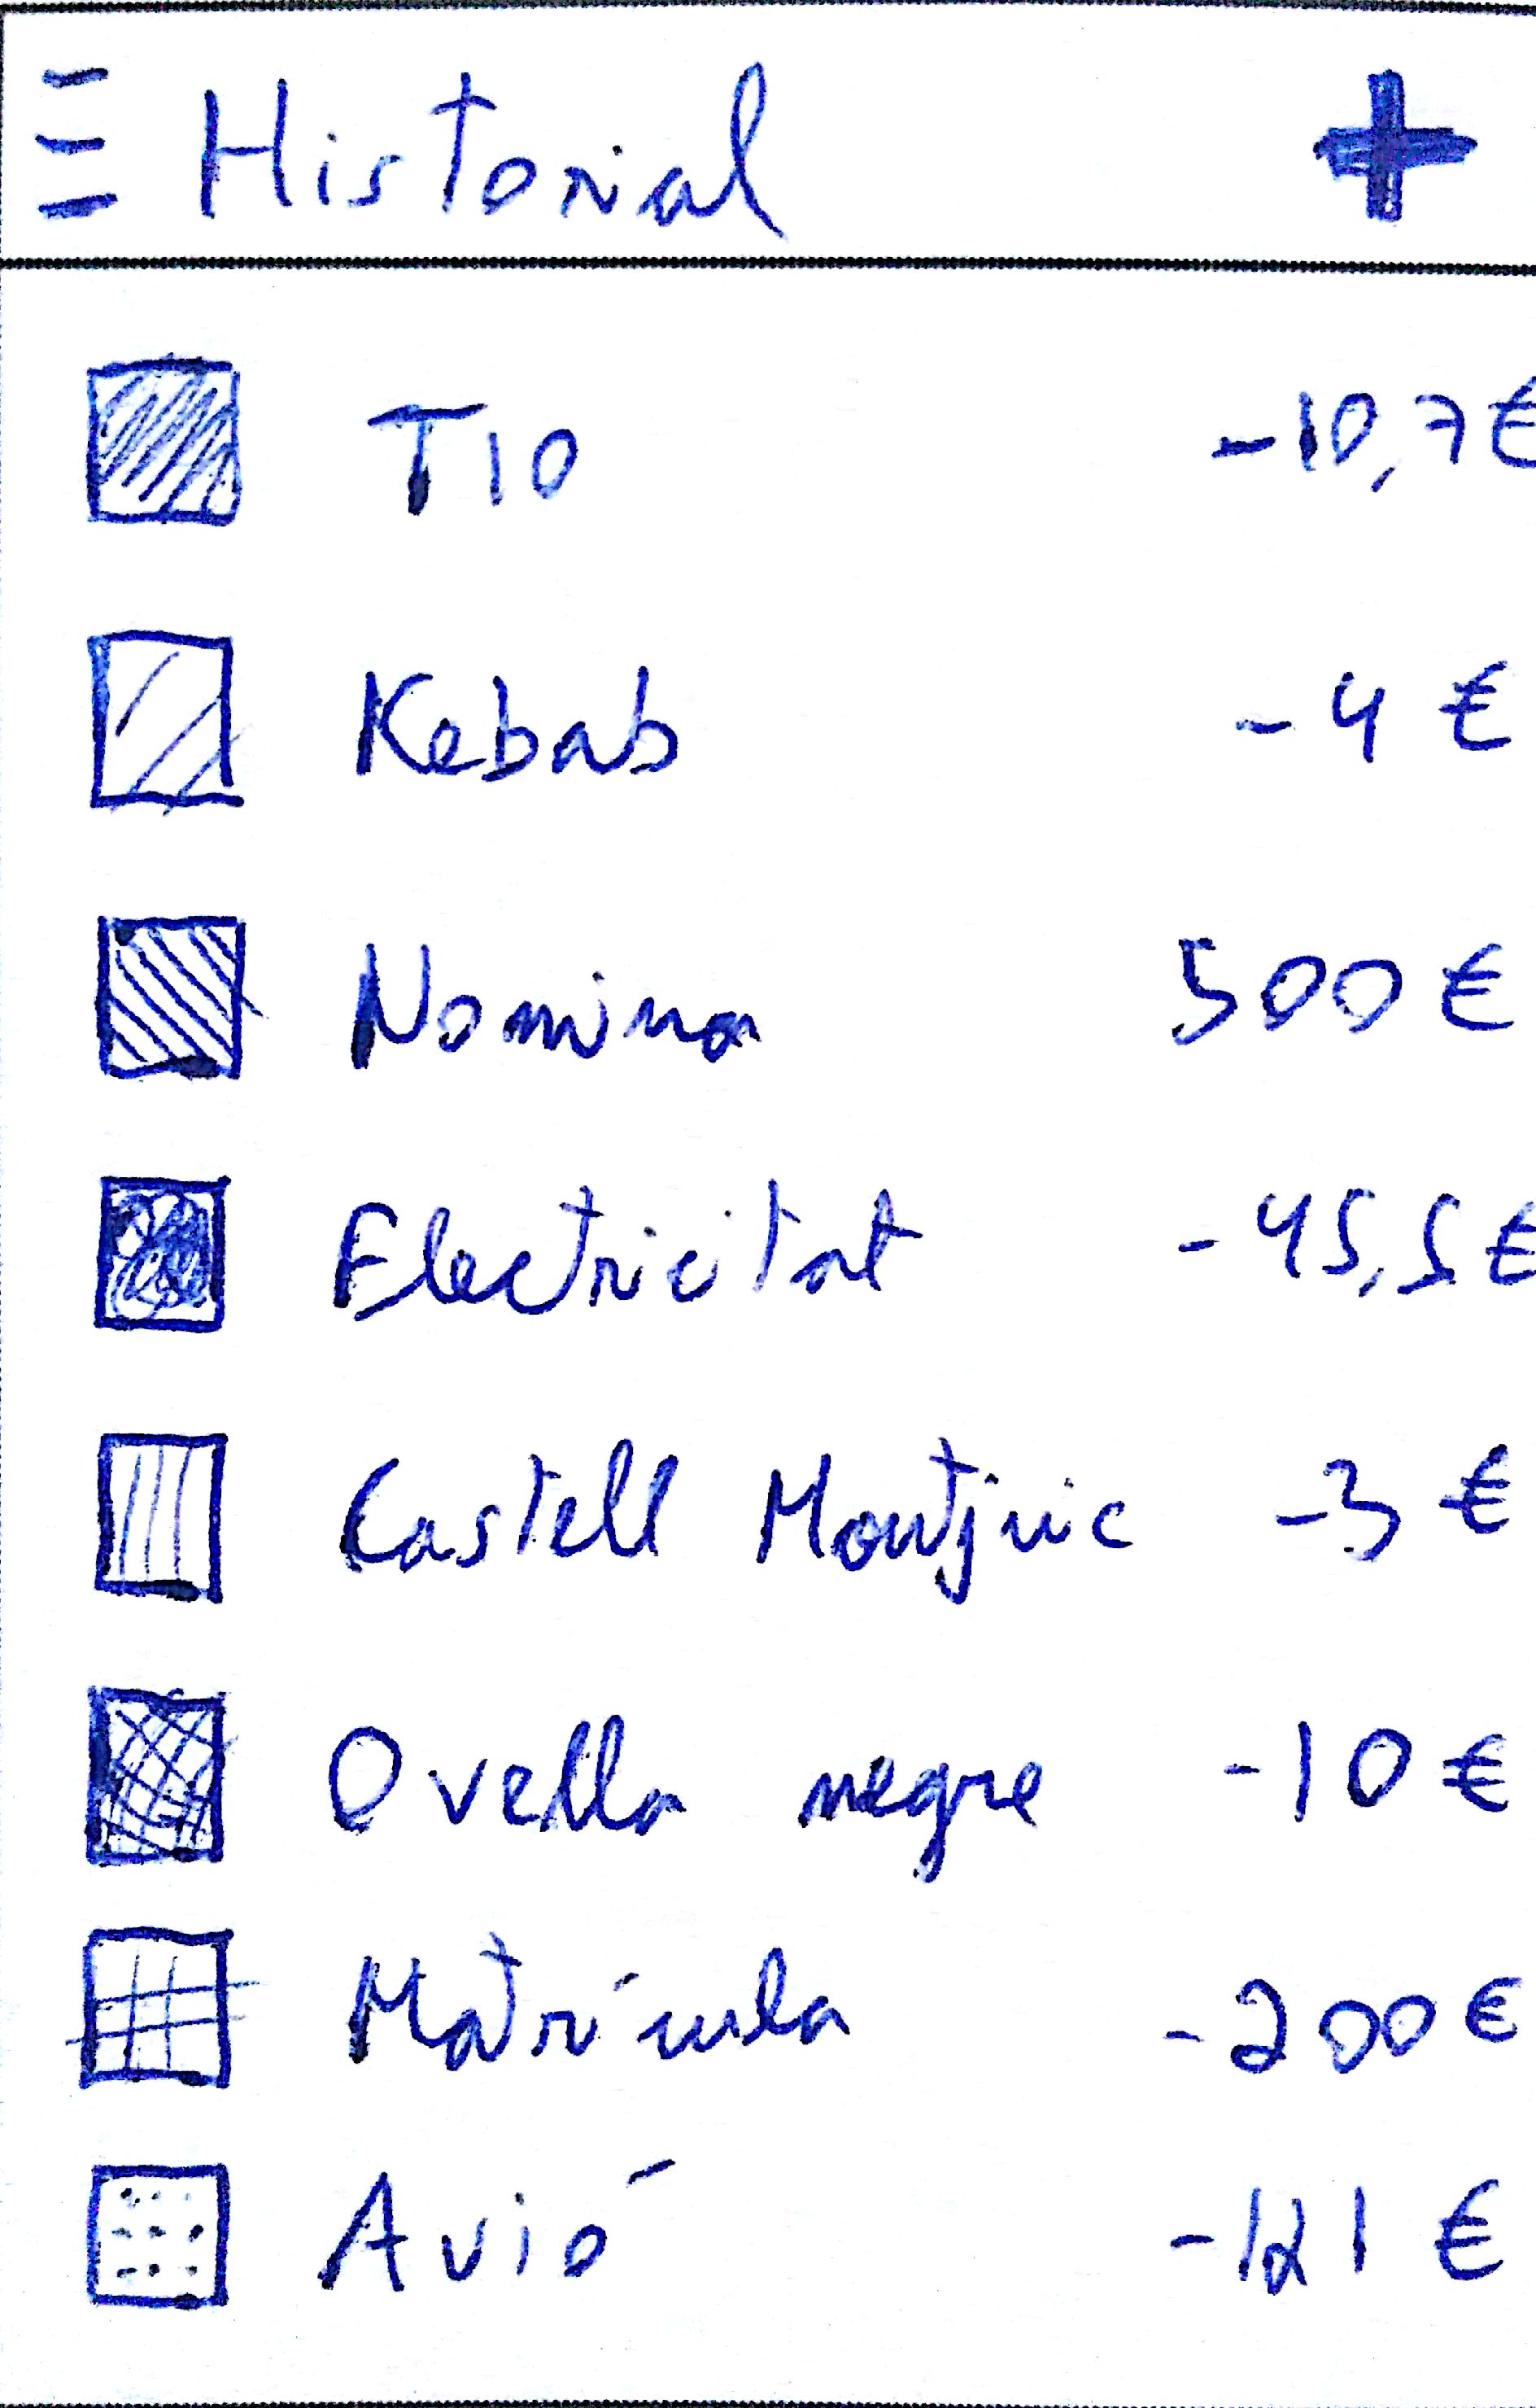
\includegraphics[width=50mm]{1_History.jpg} &
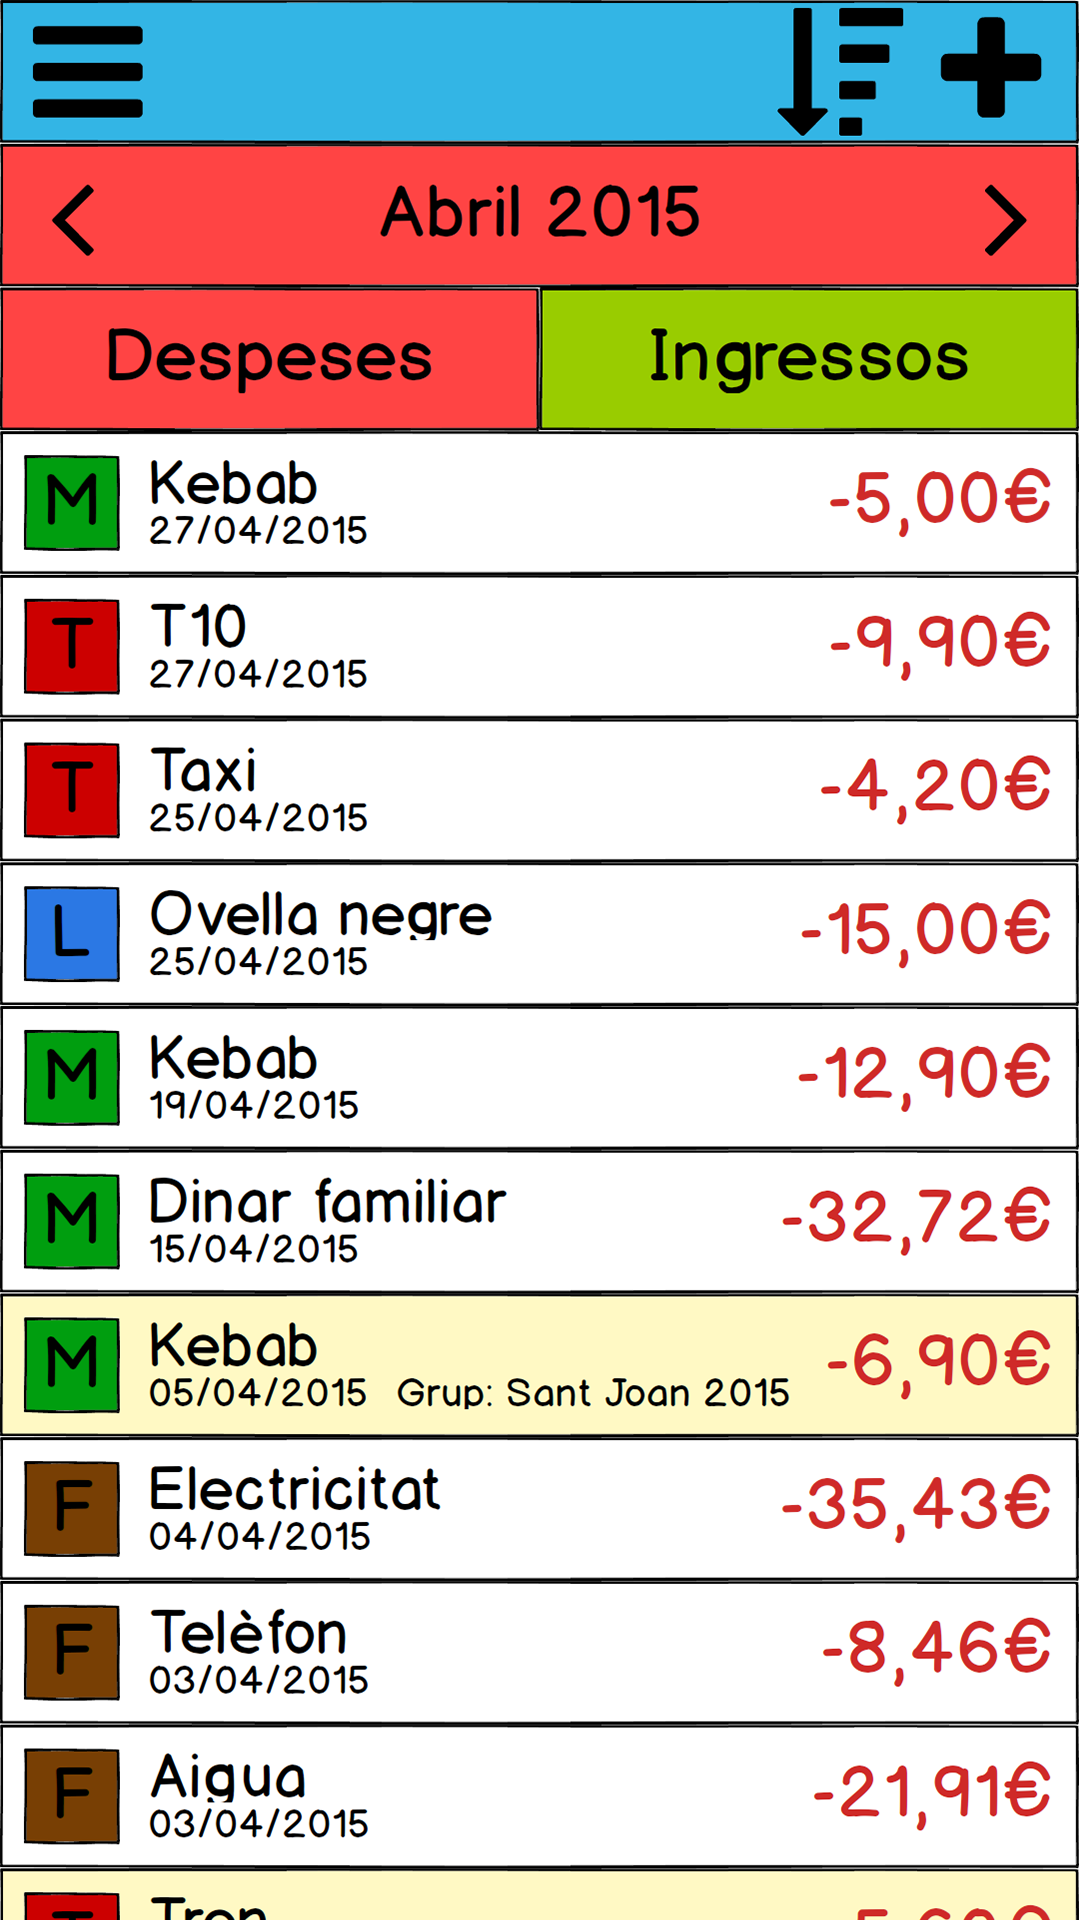
\includegraphics[width=50mm]{2_History.png} &
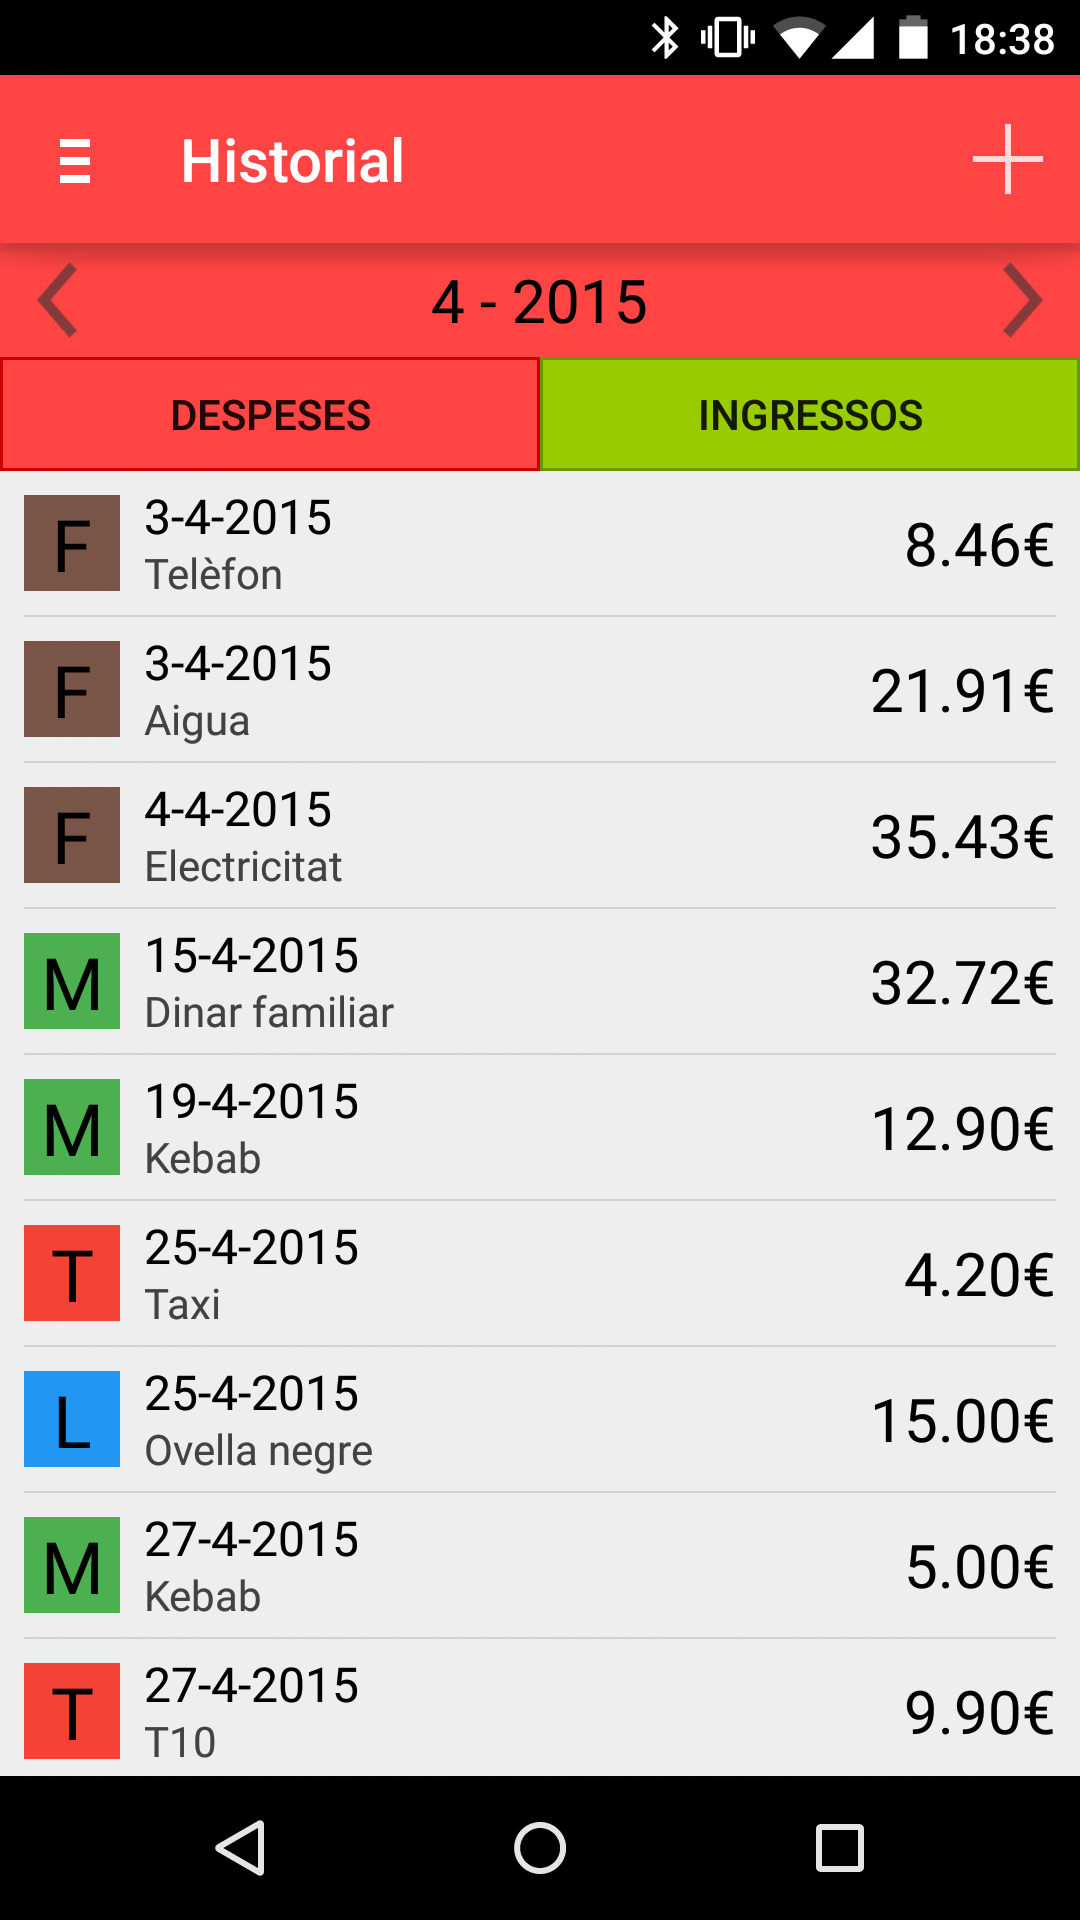
\includegraphics[width=50mm]{3_History.png}  \\
\hline
Esbossos & Disseny Conceptual - intermedi & Disseny detallat - refinat \\
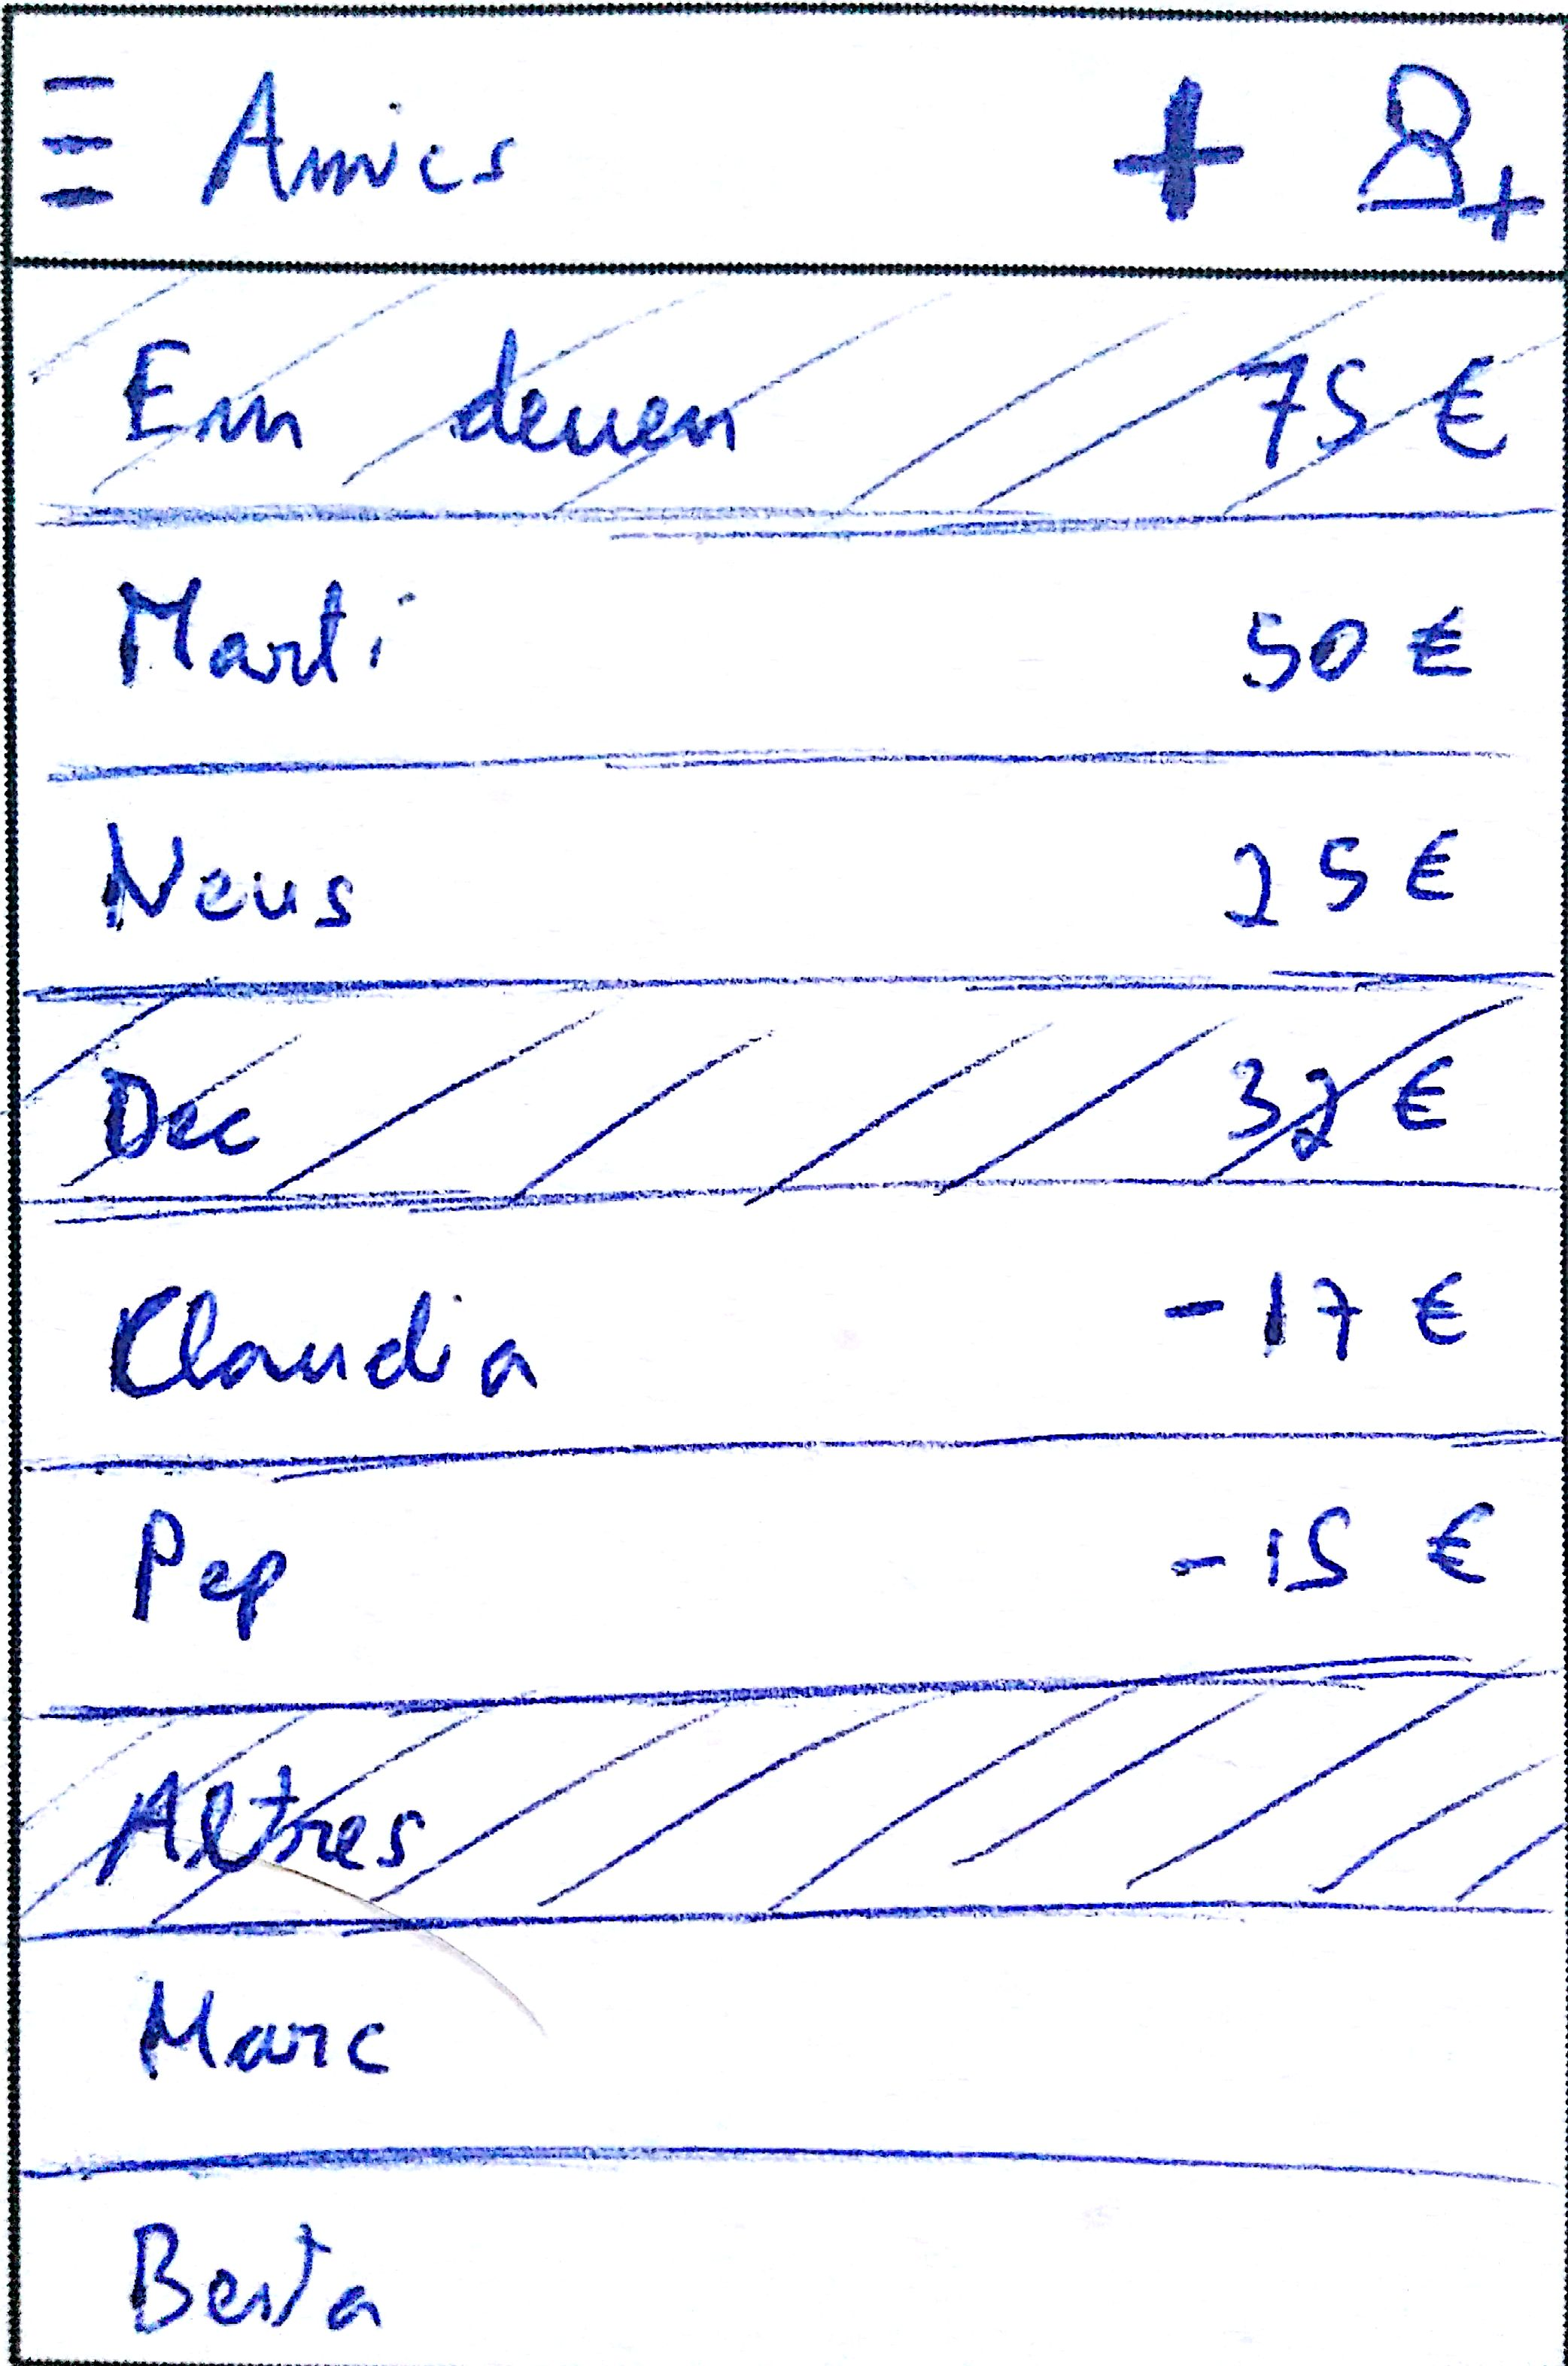
\includegraphics[width=50mm]{1_People.jpg} &
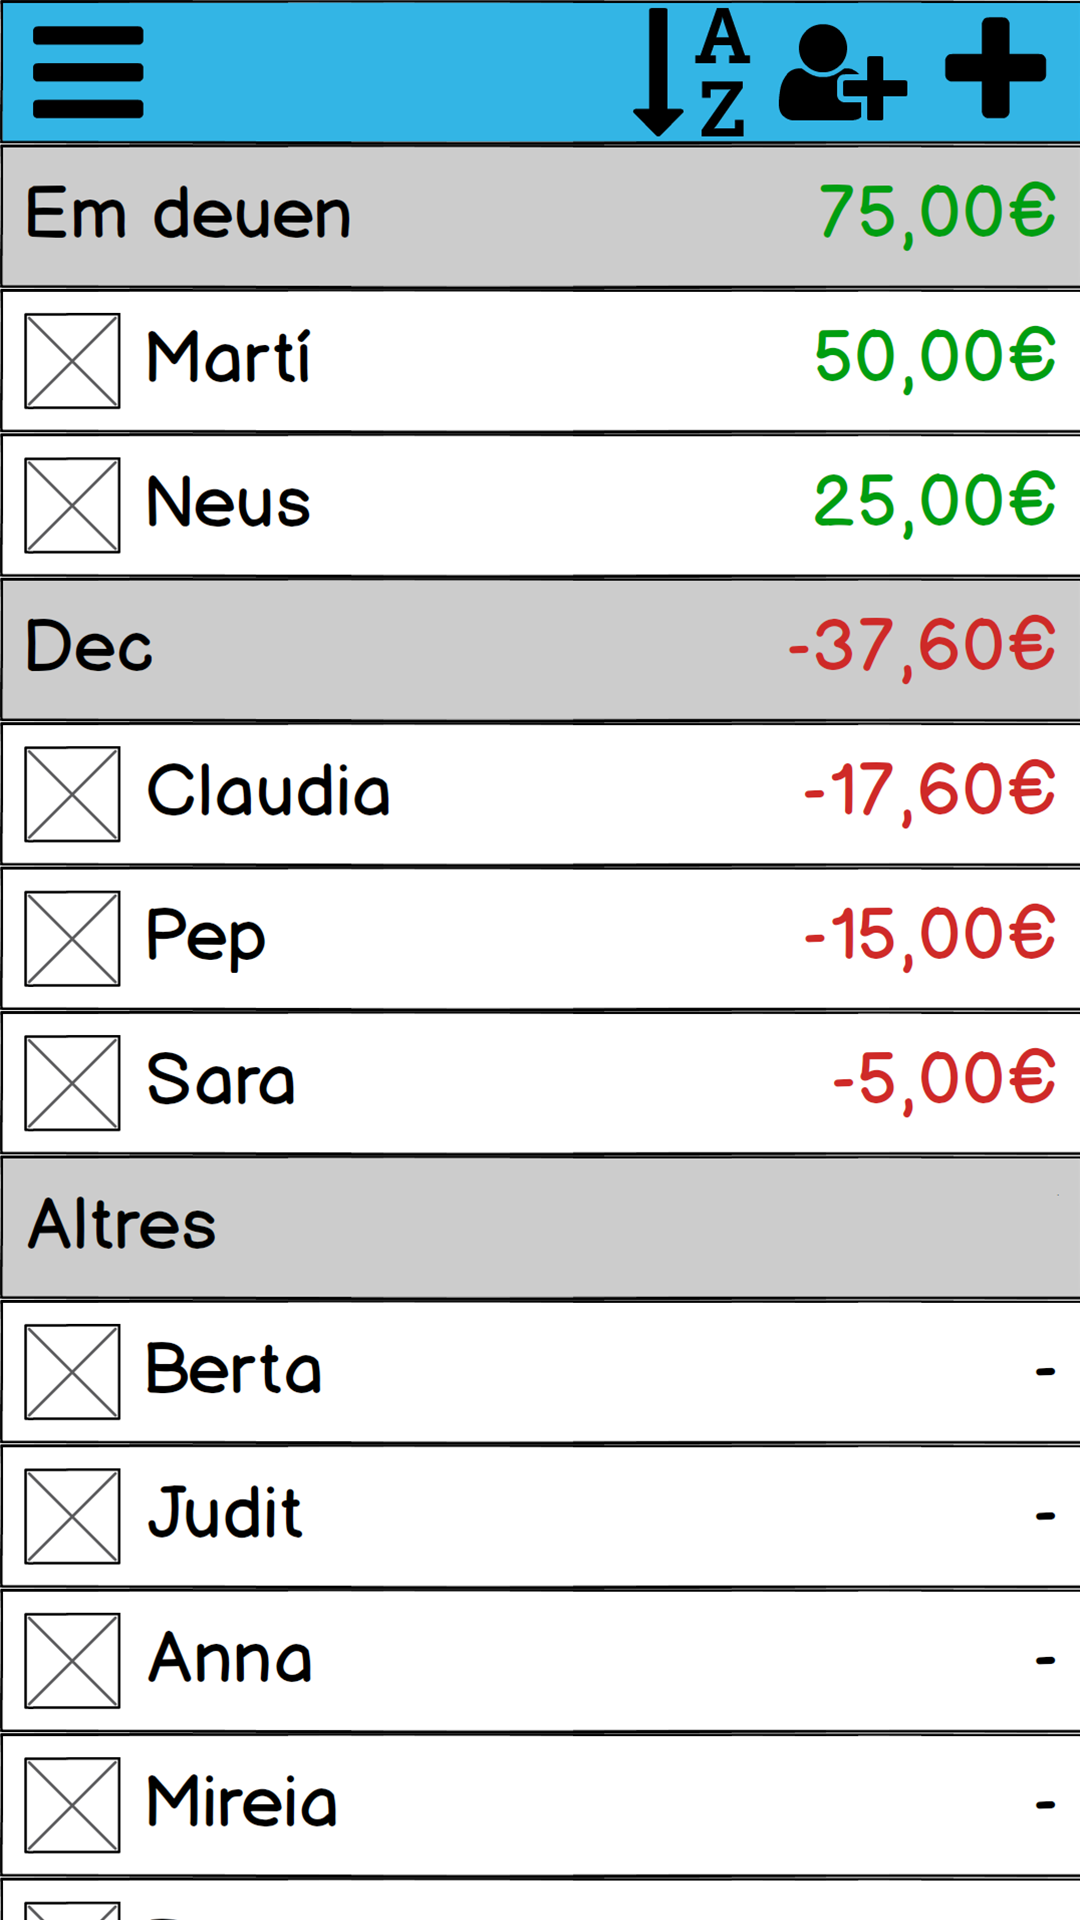
\includegraphics[width=50mm]{2_People.png} &
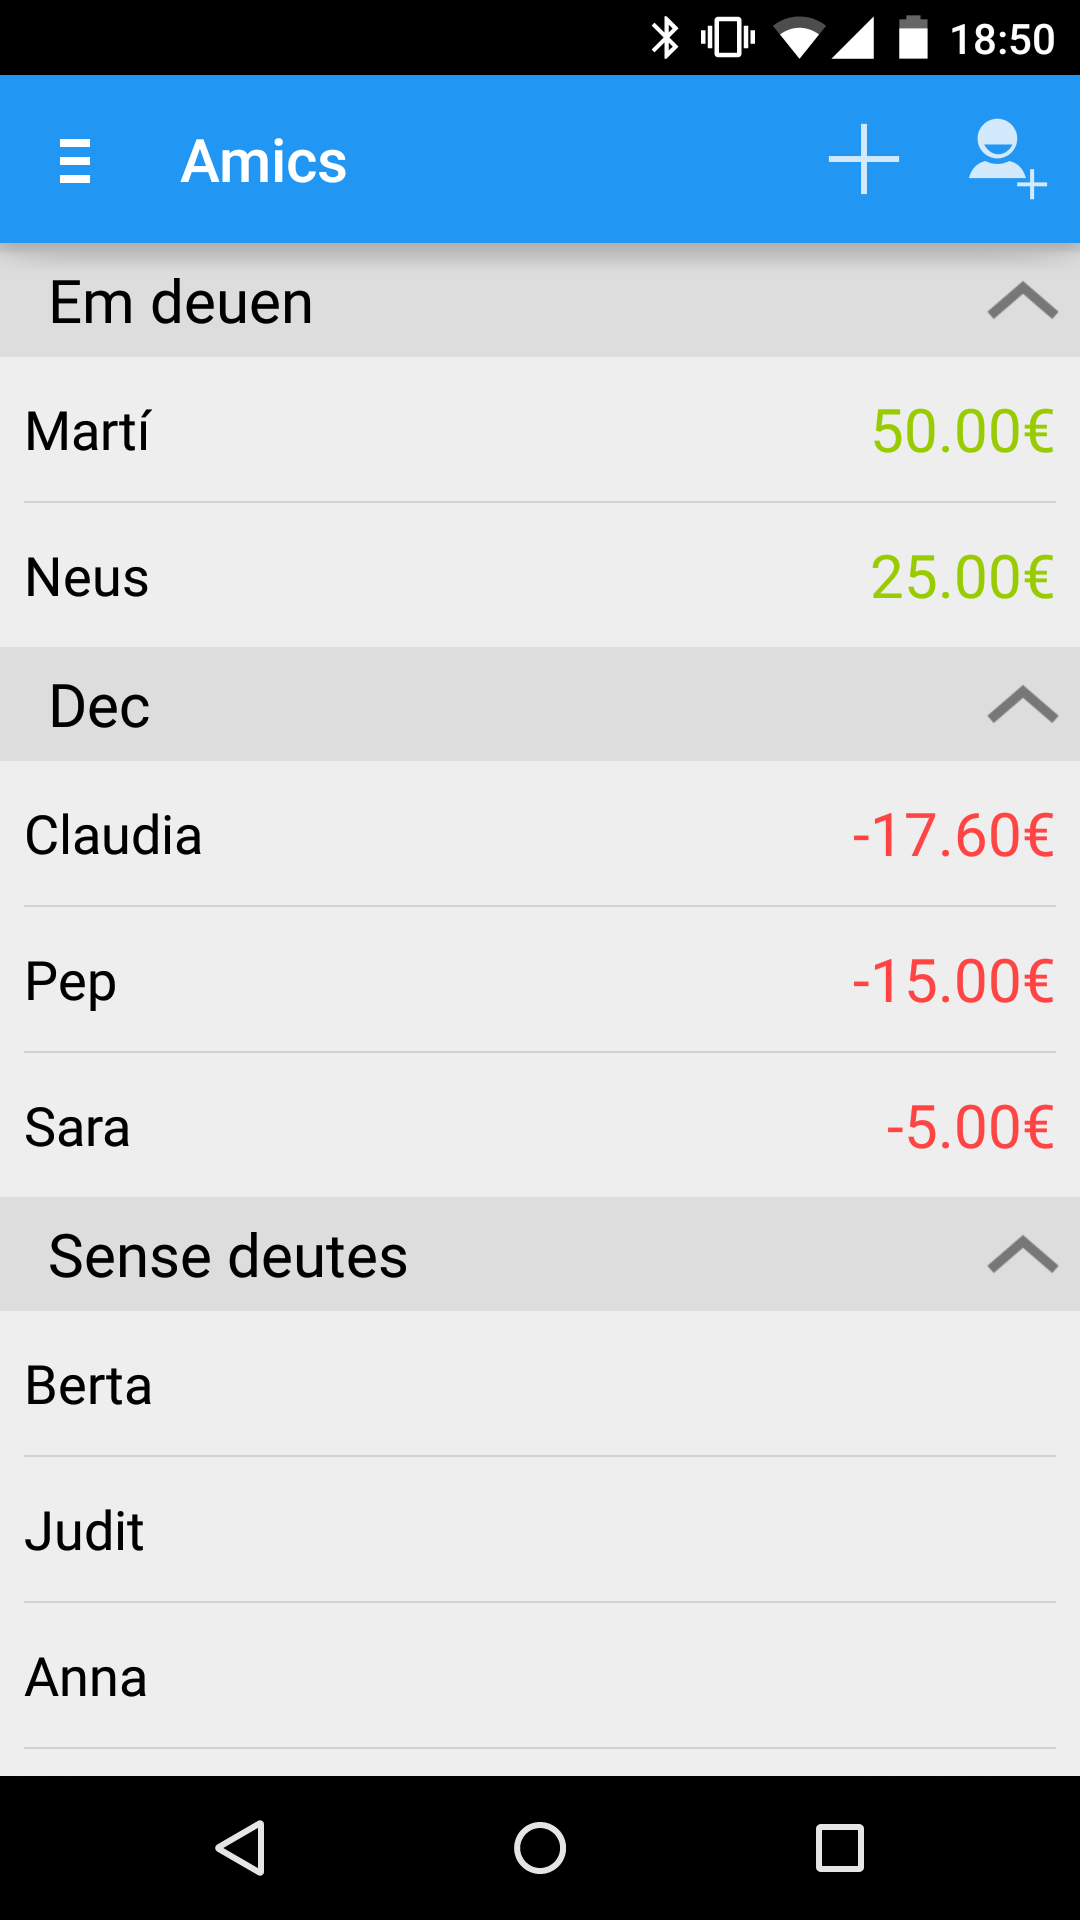
\includegraphics[width=50mm]{3_People.png}  \\
\hline
\end{tabular}
\end{table}

%TODO link a més imatges del disseny

\section{Implementació}

\begin{table}
\caption{Prototips creats}
\label{table:prototypes}
\begin{tabular}{ | p{1.6cm} | c | p{1.9cm} | l | l |}
\hline
\textbf{Codi.} & \textbf{Icona} & \textbf{Tipus de Prototip} & \textbf{Fidelitat} & \textbf{URL}\\ 
\hline
PH1 & 
\includegraphics[width=0.7cm]{PH1.png} & Horitzontal & Baixa & \href{http://invis.io/3F2TDUWP8}{http://invis.io/3F2TDUWP8} \\
\hline
PH2 & 
\includegraphics[width=0.7cm]{PH2.png} & Horitzontal & Mitja & \href{https://www.flinto.com/p/72ad65cd}{https://www.flinto.com/p/72ad65cd} \\
\hline
PV1 & 
\includegraphics[width=0.7cm]{PV1.png} & Vertical & Mitja & \href{https://www.flinto.com/p/fee8156d}{https://www.flinto.com/p/fee8156d} \\
\hline
PL1 & 
\includegraphics[width=0.7cm]{PL1.png} & Local & Mitja &  \\ %TODO link
\hline
Expensor beta & 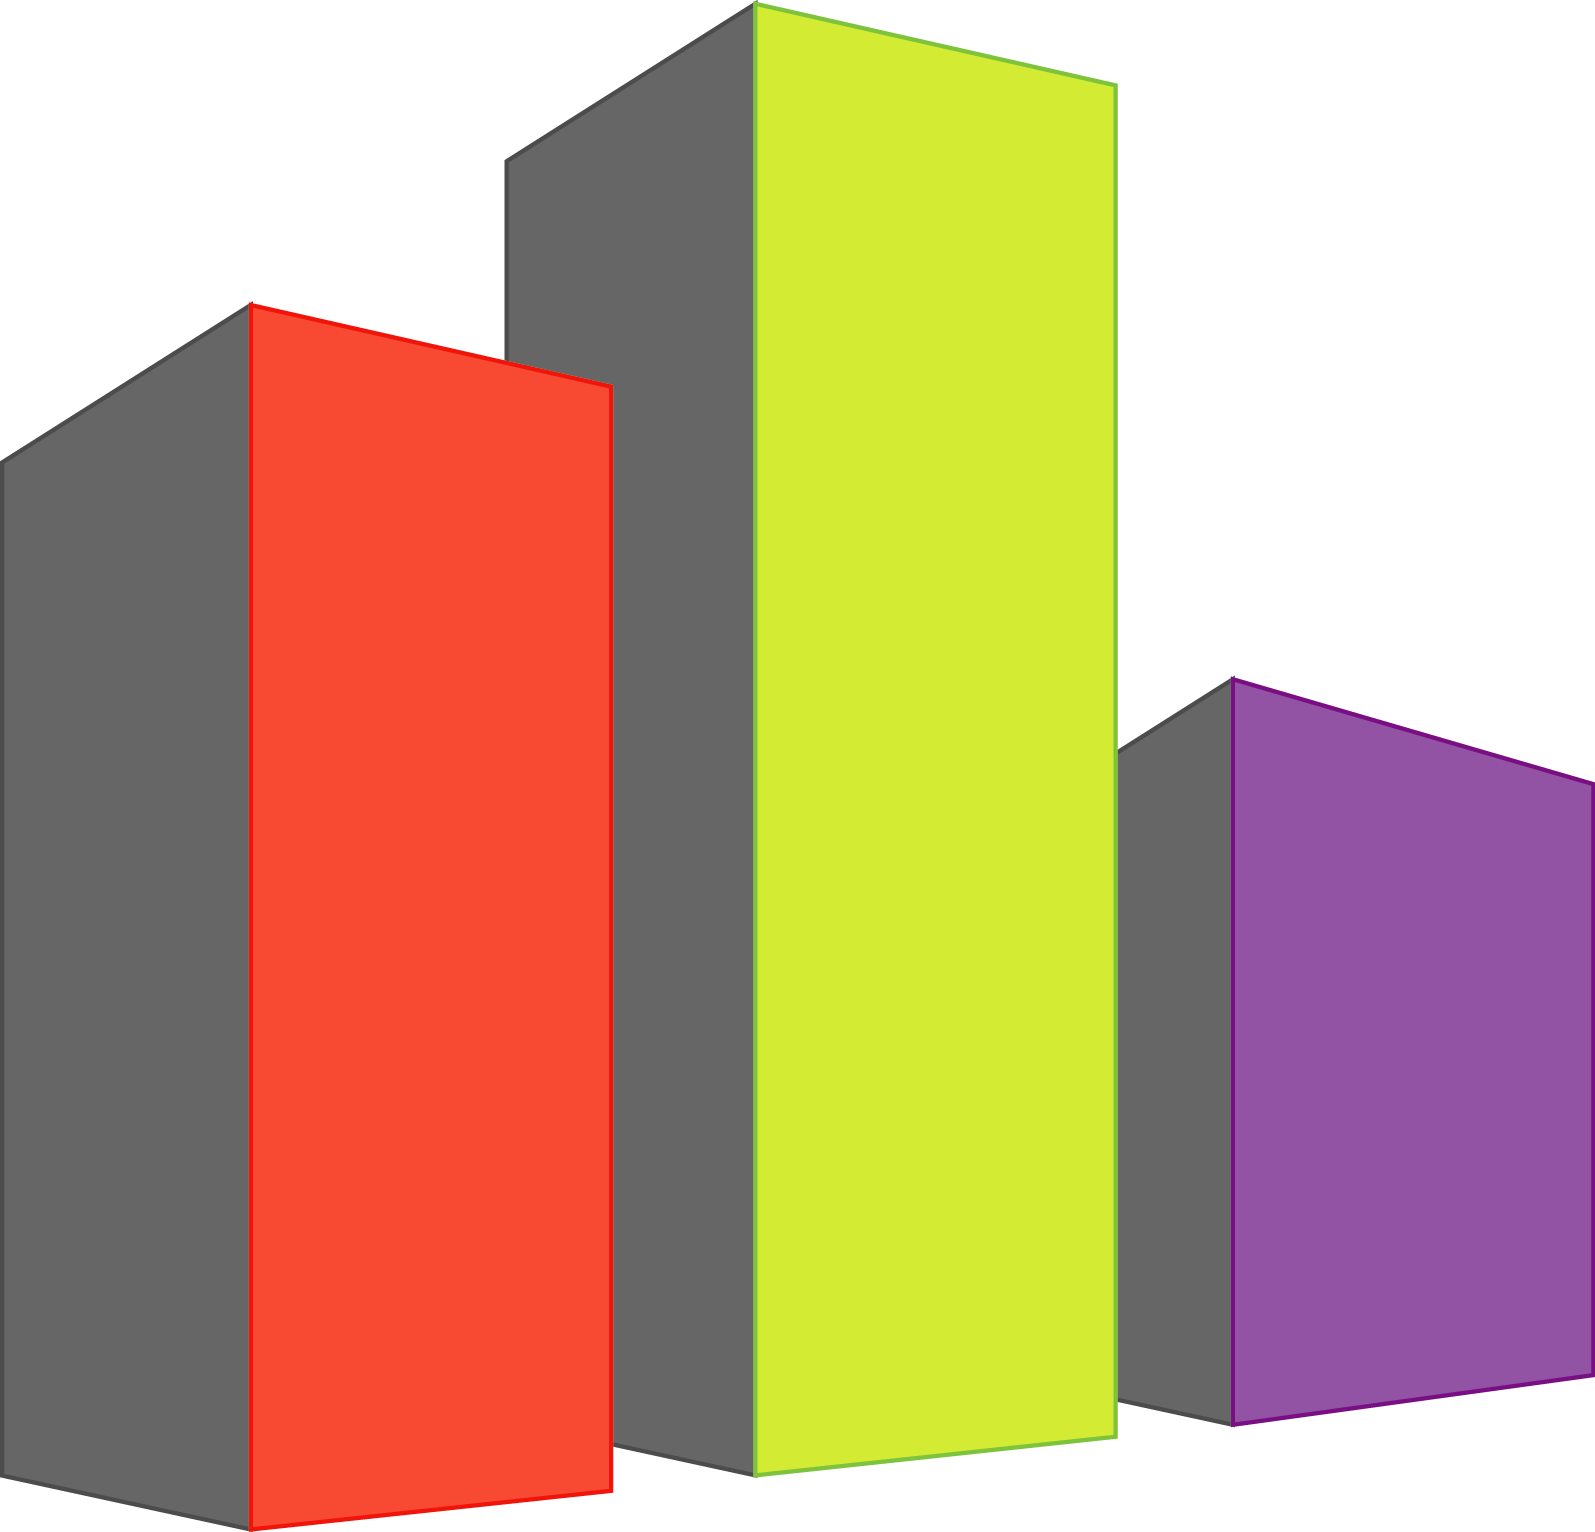
\includegraphics[width=0.7cm]{logo.png} & Complet & Alta &  \\ %TODO link
\hline
\end{tabular}
\end{table}
